\documentclass[a4paper,11pt]{article}

\usepackage[utf8]{inputenc}
\usepackage[T1]{fontenc}
\usepackage[french]{babel}
\usepackage{amsmath, amsfonts, amssymb}
\usepackage{stmaryrd}
\usepackage[french,onelanguage,boxed]{algorithm2e}
\usepackage{graphicx}
\usepackage{color}
\usepackage{dsfont}
\usepackage{subfigure}
\usepackage{geometry}
\usepackage{amsthm}
% \usepackage{fullpage}

% raccourci pour Position Du Probleme
\newcommand{\subfigPDP}[2]{
 \subfigure[#1]{\includegraphics[width=40mm]{#2}}
 }
\newcommand{\arrowPDP}{{\raisebox{15\height}{\scalebox{1}{$\longrightarrow$}}}}

%les theoremes dans le style theoreme
\theoremstyle{plain}
\newtheorem{prop}{Proposition}
\newtheorem{thm}{Théorème}
\newtheorem{lem}{Lemme}
%les theoremes dans le style definition
\theoremstyle{definition}
\newtheorem{Def}{Définition}
\newtheorem{pte}{Propriété}
\newtheorem{defnot}{Définitions et notations}
%les theoremes dans le style remarque
\theoremstyle{remark}
\newtheorem{remarque}{Remarque}
\newtheorem*{Remaffin}{Remarque sur les applications affines}

\newcommand{\affinite}[1]{\left(\begin{array}{c c|c} #1 \end{array}\right)}
\newcommand{\pmatrice}[1]{\begin{pmatrix} #1 \end{pmatrix}}

\newcommand{\pgcd}{\wedge}
\newcommand{\ppcm}{\vee}

\newcommand{\red}[1]{\textcolor{red}{#1}}
\newcommand{\blue}[1]{\textcolor{blue}{#1}}
\newcommand{\green}[1]{\textcolor{green}{#1}}

\newcommand{\Chi}{\raisebox{.40ex}{\ensuremath{\chi}}}

\newcommand{\bloc}[2]{\ \\ \underline{#1 :}\\ #2 \ \\}
\DeclareMathOperator{\sgn}{sgn}

%partieHugoraccourci
\usepackage{amsfonts}
\usepackage{graphicx}
\usepackage{stmaryrd}
\usepackage{nccmath}
\usepackage[french]{babel}
\selectlanguage{french} 
\newcommand{\A}[0]{{\cal A}}
\newcommand{\C}[0]{{\cal C}}
\newcommand{\se}[1]{\medbreak \medbreak \section{#1}}
\newcommand{\sse}[1]{\medbreak \subsection{#1}}
\newcommand{\ssse}[1]{\subsubsection{#1}}
\newcommand{\sssse}[1]{\paragraph*{#1}}
%\newcommand{\Def}[0]{\ssse{Définition}}
\newcommand{\The}[0]{\ssse{Théorème}}
\newcommand{\Pro}[0]{\ssse{Propriété}}
\newcommand{\Exo}[1]{\sse{Exercice #1}}
\newcommand{\Que}[1]{\ssse{Question #1}}
\newcommand{\llb}[0]{\llbracket}
\newcommand{\rrb}[0]{\rrbracket}
\newcommand{\dd}[0]{\txt{d}}
\newcommand{\ssi}[0]{\Leftrightarrow}
\newcommand{\ra}[0]{\rightarrow}
\newcommand{\Ra}[0]{\Rightarrow}
\newcommand{\la}[0]{\leftarrow}
\newcommand{\La}[0]{\Leftarrow}
\newcommand{\txt}[1]{\textrm{#1}}
\newcommand{\ol}[1]{\overline{#1}}
\newcommand{\ul}[1]{\underline{#1}}
\newcommand{\mb}[1]{\mathbb{#1}}
\newcommand{\abs}[1]{|#1|}
\newcommand{\iso}[0]{\simeq}
\newcommand{\dr}[0]{\partial}
\newcommand{\floor}[1]{\lfloor #1\rfloor}
 \newcommand{\BlockIf}[1]{\KwSty{Start If} \\ #1 \\ \KwSty{End If}}
 \newcommand{\BlockElseIf}[1]{\KwSty{Start Else If} \\ #1 \\ \KwSty{End Else If}}
 \newcommand{\BlockElse}[1]{\KwSty{Start Else} \\ #1 \\ \KwSty{End Else}}
\usepackage[french,onelanguage]{algorithm2e}
%finpartie



\newenvironment{algorithme}{\begin{algorithm}[H]}{\end{algorithm}}



\DeclareMathOperator{\supp}{supp}
\DeclareMathOperator{\sinc}{sinc}
\DeclareMathOperator{\Sp}{Sp}
\DeclareMathOperator{\Tr}{Tr}



% \setcounter{secnumdepth}{5} % ajouter des \paragraph et \subparagraph
% \setcounter{tocdepth}{5} % pour que les \paragraph et \subparagraph apparaissent au sommaire



\begin{document}
   	\begin{titlepage}
	\begin{center}
	\vspace*{\fill}

		\vspace{0.3cm}
		{\huge Titre}\\
		\vspace{1.5cm}
	\today
	\vspace{1.5cm}


		\large
			\emph{Auteurs:}\\
			Simon Barazer,\\
			Jean-Thomas De La Roche Saint-André,\\
			Hugo Moeneclaey, \\
			Shmuel Rakotonirina--Ricquebourg
		
\medbreak
\medbreak
\medbreak
\medbreak
\medbreak
\medbreak

		\large
			\emph{Sous la direction de:}\\ 
			Jean-Michel Morel \\
			Enric Meinhardt-Llopis
		


	\vfill
	\end{center}
   	\section*{Résumé}
   		% contient l'abstract
This article presents a new methode of image resampling by an homography by spliting it into three mappings. Two of them are affine transforms which are easier to resample than an homography. The last mapping is a special homography : an unidirectional homography, which means that it conserves verticals. The unidirectional homography is interesting because it splits itslef into two unidimensional mappings (which resamples each rows or each columns independently). This new method is compared with pre-existing methods, such as the Ripmap.





%Cet article présente une nouvelle méthode de ré-échantillonnage d'une image par une homographie en décomposant cette dernière en plusieurs transformations, affines et homographiques. En passant par des affinités qu'on peut traiter de manière bien plus efficace que les homographies, on se ramène donc au traitement d'une famille d'homographies particulières : ces homographies seront unidirectionnelles, au sens où elles conservent les verticales, et pourront se décomposer en deux applications unidimensionnelles (qui traitent chaque ligne ou chaque colonne indépendamment). Les résultats obtenus en utilisant cette décomposition sont comparés avec les méthodes déjà existantes, notamment le Ripmap.


	\end{titlepage}
	\tableofcontents
		\section*{Remerciements}
		% On met les remerciements

We would like to express our gratitude to Jean-Michel Morel and Enric Meinhardt-Llopis for having taken care of us during our internship.
%Merci à Jean-Michel Morel et à Enric Meinhardt-Llopis pour nous avoir si bien encadrés durant notre stage.
 %Jean-Thomas
	\section*{Introduction}%Jean-Thomas
		% contient l'introduction
	La première partie de cet article (cf partie \ref{Exposition_du_probleme}) traite du problème des homographies en général et fait une présentation non-exhaustive des méthodes actuelles pour traiter les homographies. Elle présente aussi une méthode de traitement des affinité que nous utilisons dans notre méthode de traitement des homographies.

	La seconde partie (cf partie \ref{decomp_geo_hom} ) présente une interprétation géométrique d'une homographie en terme de mouvement de caméra. Elle permet de comprendre la théorie qui justifie notre méthode.

	La partie expérimentale (cf partie \ref{experiences}) montre les performances et le gain en qualité de notre méthode de traitement des homographies par rapport aux méthodes existantes (comme le Ripmap par exemple).

	Les pseudo-codes permettant de mettre en oeuvre notre méthode sont présents en annexe.

	\section{Exposition du problème}
		\label{Exposition_du_probleme}
		\subsection{Position du problème}
			% contient une exposition du problème (description d'une homographie, source du problème, intérêt du problème, problématique, raison pour laquelle on se bat dans la vie, etc...)
%Jean-Thomas
		\subsection{Méthodes existantes}
			% contient une explication du fonctionnement du Mip Map et du Rip Map, et des schémas explicatifs. En bref, un résumé de l'article de Williams
% parler éventuellement de la méthode naïve, ou d'autres méthodes actuelles qui ne fonctionnent pas



\ssse{Méthode naïve}

%petite explication de la méthode naive, puis :

\begin{figure}[h!]
\centering
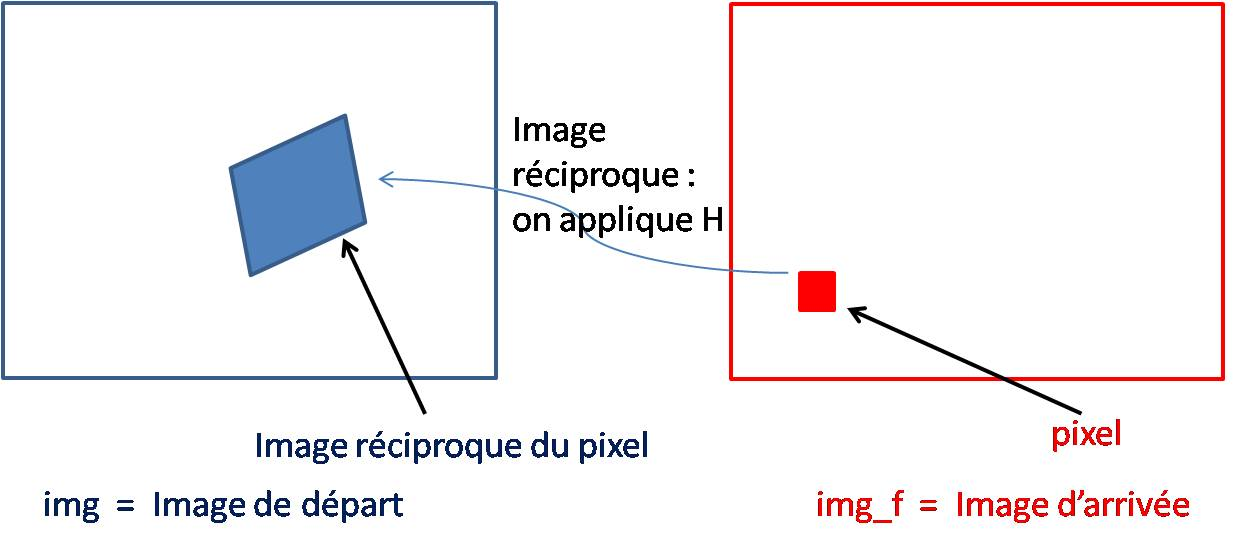
\includegraphics[scale=0.5]{imagereciproque.jpg}
\caption{Image réciproque d'un pixel}
\end{figure}

En pratique on utilise plutôt le Mipmap. C'est une méthode utilisée en texturing, présentée par Williams en 1983.

\ssse{Principe}

Le principe est de précalculer des coefficients qui représentent des zones entières de l'image, pour pouvoir ensuite calculer en temps réel une homographie. 

Pour cela on choisit de supposer que l'image est carrée de taille une puissance de 2 (quitte à faire un premier zoom). On calcule ensuite la valeur de certains carrés de l'image de taille une puissance de 2.
Le Mipmap est donc représenté par une suite d'image chacune deux fois plus petite que la précédente, qui sont des "zoom-out" de l'image d'origine de facteur une puissance de 2.

%image d'un vrai mipmap, que je ferais moi
\begin{figure}[h!]
\centering
\caption{Un exemple de Mipmap}
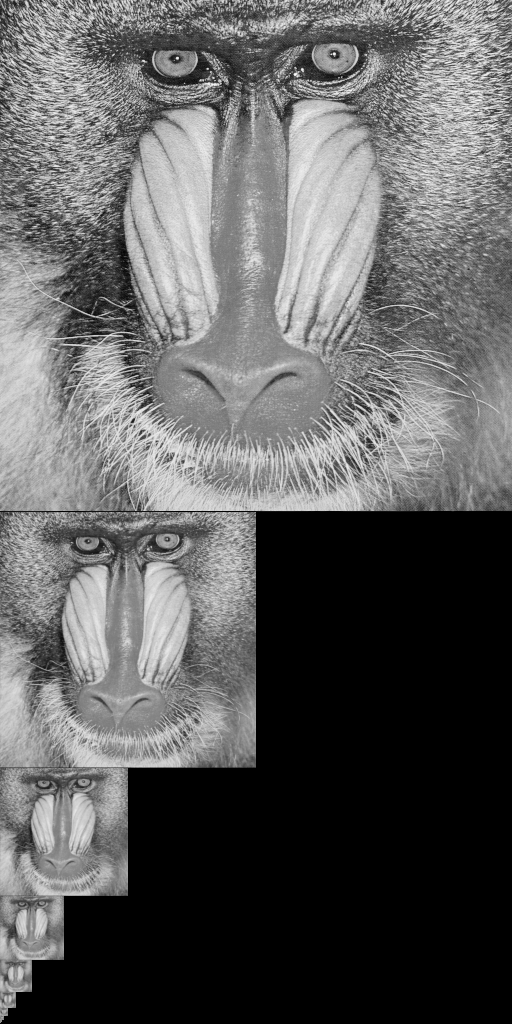
\includegraphics[scale=0.4]{MipMap_real} %scale=0.4 ça fait vachement petit, non ?
\end{figure}

Ensuite, quand on cherche la valeur d'un pixel de l'image d'arrivée, on regarde la zone de l'image de départ à laquelle il correspond à l'aide des différentielles de l'homographie inverse. On obtient alors approximativement un parallélogramme, qu'on essaye d'approximer par des carrés.

%image de parallélogramme avec les différentielles, avec au mieux schéma image de départ / arrivé qui explique la correspondance entre un pixel est un parallélogramme

On appelle distance la taille d'un carré (car plus un pixel est "loin", plus les carrés qui l'approximent sont grands). 

On suppose avoir une formule nous donnant la distance d'un point quelconque, la géométrie du Mipmap ne permettant que des distances puissance de 2, on fait une approximation trilinéaire : 

\begin{itemize}
  \item d'une part, on fait une interpolation linéaire entre deux niveaux de profondeur qui encadrent la distance.
  \item d'autre part, dans chaque niveau du Mipmap, on fait une interpolation bilinéaire entre les quatre carrés où tombe le pixel.
\end{itemize}

%image de l'inter trilinéaire avec deux plans pour les profondeurs
\begin{figure}[h!]
\centering
\caption{Schéma d'interpolation trilinéaire}
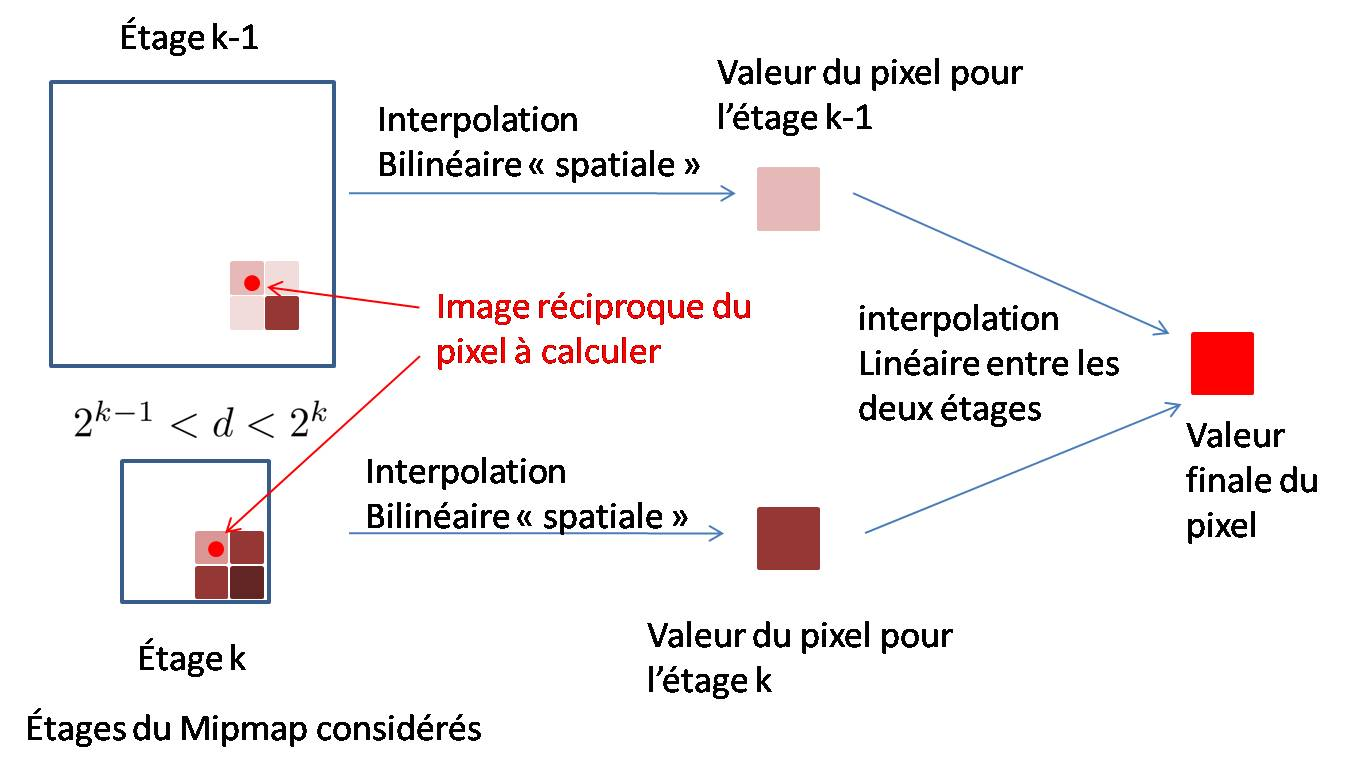
\includegraphics[scale=0.5]{intertrilineaire.jpg}
\end{figure}

\ssse{La fonction de distance}

Toutes les fonctions de distance dépendent de la différentielle de l'homographie inverse.
On note $(u,v)$ les coordonnées dans l'image d'origine et $(x,y)$ celles dans la fenêtre d'arrivée.

Il est aisé de calculer les coefficients des dérivées partielles. On note $H$ l'homographie inverse.

%re image prgm, avec les dérivé partielle indiqués

L'enjeu est que si $d$ est trop grand, l'image est inutilement floutée (on parle d'\emph{over-blurring}), et si $d$ est trop petit l'image est aliasée.

% On a jugé de la performance des méthodes "à vue". On compte à terme l'évaluer sur des cosinus/sinus.

On note $\dd_{(x,y)} H$ la différentielle de $H$ en $(x,y)$.

On note $(u,v)=H(x,y)$.

\sssse{Méthode du déterminant}
$$D(x,y) = \sqrt{\det \txt{d}_{(x,y)} H}$$
En effet le déterminant est l'aire du parallélogramme, donc prendre un carré de coté la racine donne un carré de même aire.

Le résultat est relativement satisfaisant.

%schéma avec un ârallélogramme et le carré correspondant

\sssse{Méthode du plus grand côté}
$$ D(x,y) = \max \left(\sqrt{\left(\frac{\dr u}{\dr x}\right)^2 + \left(\frac{\dr v}{\dr x}\right)^2},\sqrt{\left(\frac{\dr u}{\dr y}\right)^2 + \left(\frac{\dr v}{\dr y}\right)^2}\right)$$
On prend le plus grand côté du parallélogramme comme côté du carré. Le résultat est bon. Cette formule viens d'un article de Heckbert \cite{heckbert1983texture}.

Ce résultat est satisfaisant.

%schéma avec un ârallélogramme et le carré correspondant

\sssse{Méthode des diagonales}
$$D(x,y) = \max \left( \sqrt{\left(\frac{\dr v}{\dr x}-\frac{\dr  u}{\dr  x}\right)^2+\left(\frac{\dr v}{\dr y}-\frac{\dr  u}{\dr y}\right)^2}, \sqrt{\left(\frac{\dr u}{\dr x}+\frac{\dr  v}{\dr  x}\right)^2+\left(\frac{\dr u}{\dr y}+\frac{\dr  v}{\dr  y}\right)^2} \right)$$
On prend la plus grande diagonale du parallélogramme. Ici l'image est trop flou.

%schéma avec un parallélogramme et le carré correspondant

\sssse{Méthode des valeurs singulières}

On peut décomposer toute matrice $A$ en trois matrices $A = PDQ^{-1}$ où $P$ et $Q$ sont orthogonales et $D$ est diagonale.

Pour cela on diagonalise $AA^t$, et $A^tA$, on prend $P$ et $Q$ des vecteurs propres normalisés de ces matrices, et $D$ la racine de leur diagonalisée. Il faut veiller à ce que $P$ et $Q$ correspondent bien \cite{abdi2007singular}.

Les coefficients de $D$ sont appelés valeurs singulières de $A$. On prend $D(x,y)$ le maximum des deux valeurs singulières de $A$.

Rq : On a une interprétation géométrique à l'aide d'une caméra de ces valeurs.

\sssse{Conclusion}

Les méthode du déterminant, du maximum des côtés et des valeurs singulières sont satisfaisantes.

On a une préférence pour le plus grand côté et la valeur singulière, en effet le déterminant semble introduire un peu plus d'aliasing. 

\ssse{Algorithme amélioré : Le ripmap}

Une des grandes faiblesses est l'anisotropie du Mipmap : il ne privilégie aucune direction. Ainsi si le parallélogramme à approximer et en fait un rectangle très plat, il n'y a pas d'approximation raisonnable à l'aide d'un carré.

Pour tenter de palier à ce problème on utilise un ripmap \cite{akenine2008real}. C'est en fait un Mipmap où l'on a aussi calculé la moyenne des pixels de tous les rectangles dont les côtés sont des puissances de deux.

Ainsi la fonction de distance ne renvoie plus une valeur mais deux, une pour chaque côté du rectangle. On réalise alors une interpolation bi-bi-linéaire (bilinéaire entre les niveaux et bilinéaire dans chacun d'eux).

%un vrai ripmap, que je ferais moi
\begin{figure}[h!]
\centering
\caption{Un exemple de Ripmap}
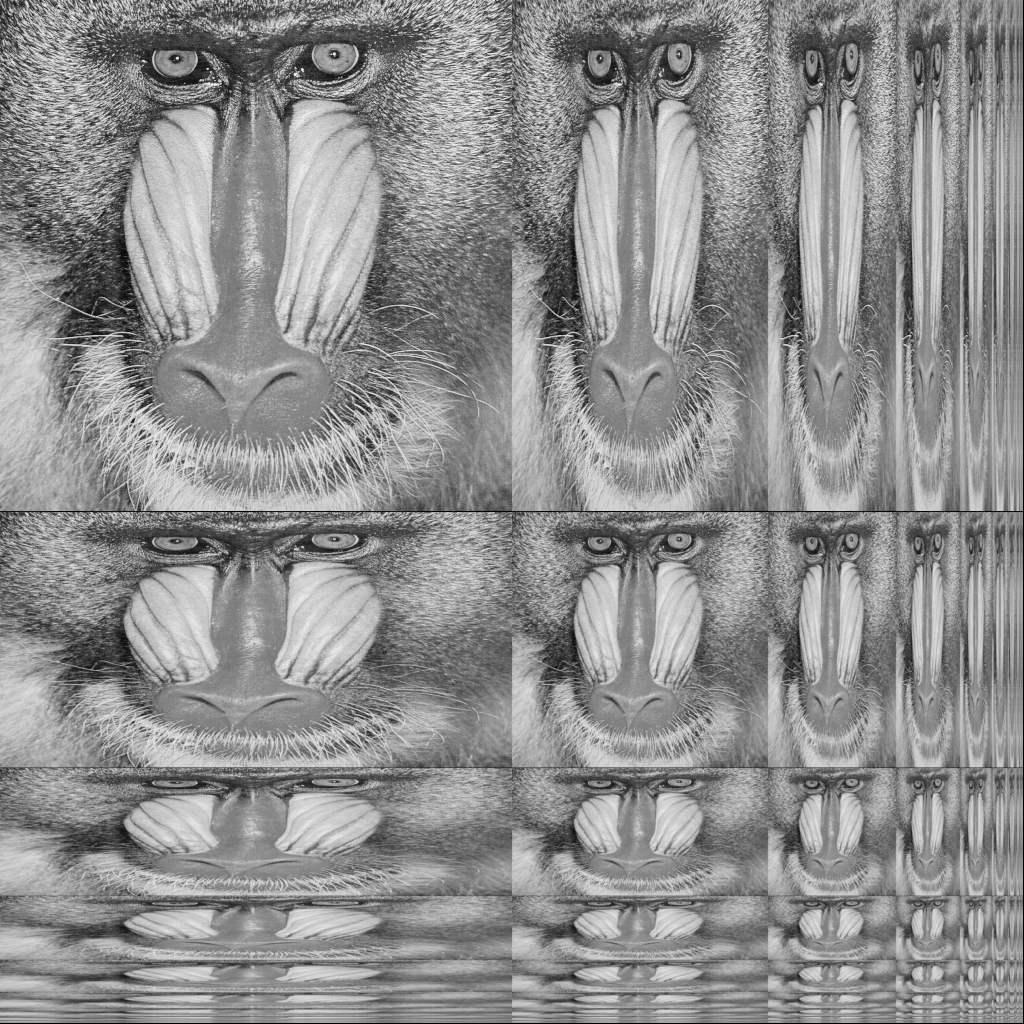
\includegraphics[scale=0.4]{Ripmap_real}
\end{figure}


%schéma d'interpolations pour le ripmap, avec 4 images est l'endroit ou le point tombe dans chacun
\begin{figure}[h!]
\centering
\caption{Schéma d'interpolation bi-bi-linéaire}
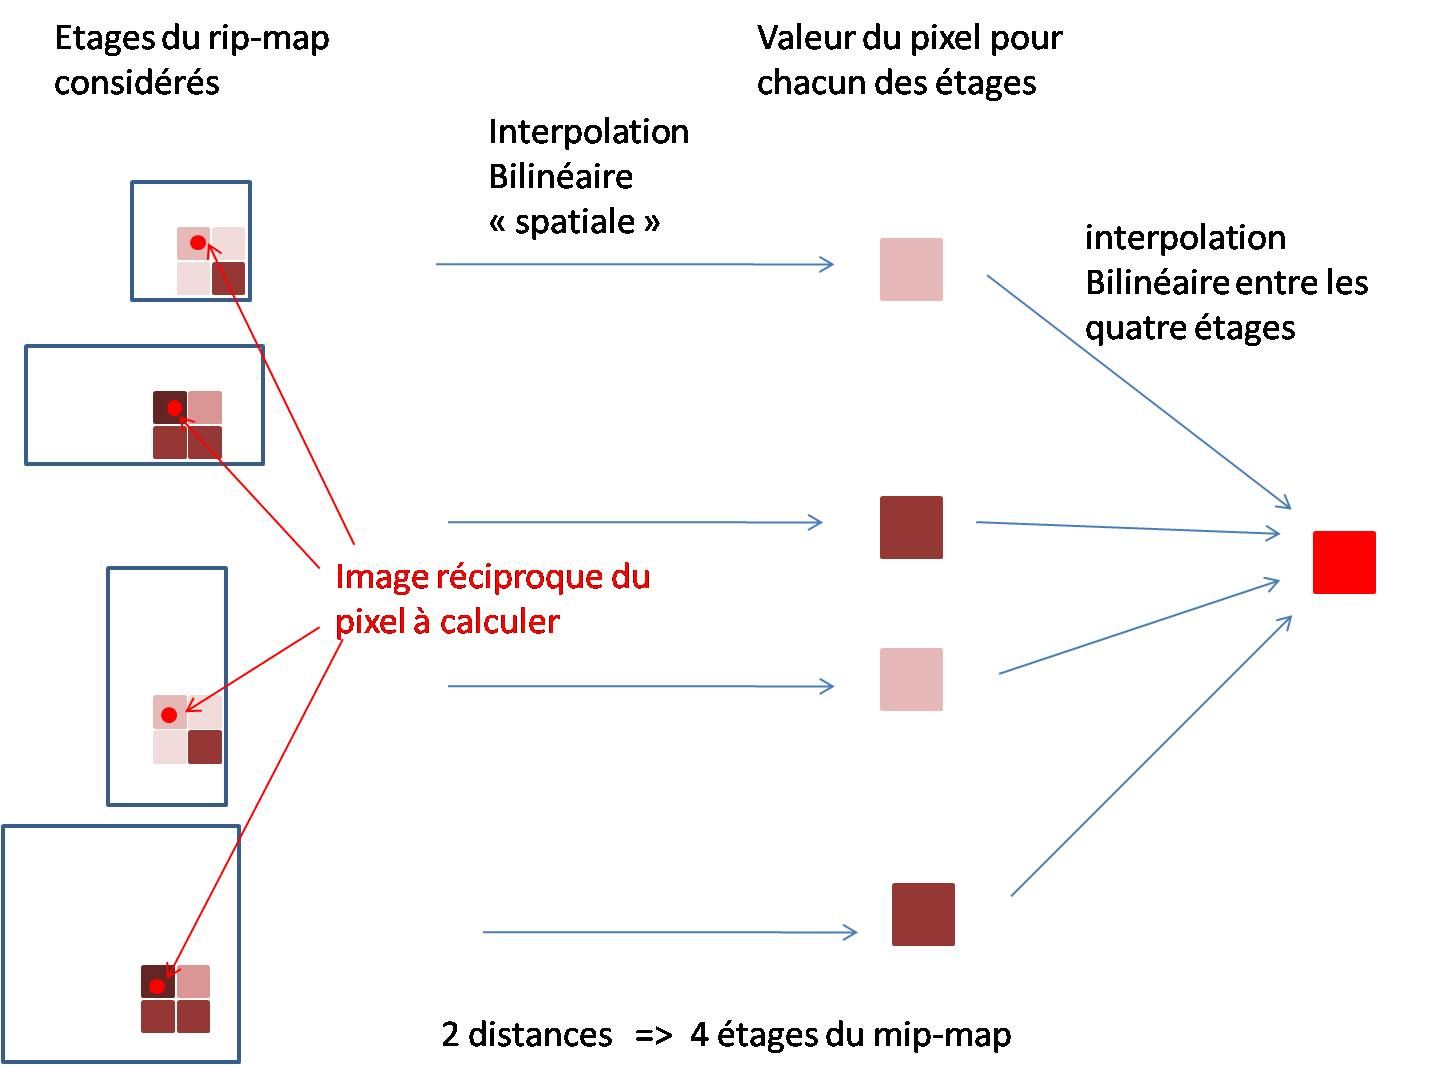
\includegraphics[scale=0.5]{interbibilineaire.jpg}
\end{figure}


On a utilisé le plus petit rectangle qui contient le parallélogramme. Ainsi la formule est de :
$$D(x,y) = \left( |\frac{\dr u}{\dr x}|+|\frac{\dr u}{\dr y}|,|\frac{\dr v}{\dr x}|+|\frac{\dr v}{\dr y}|\right)$$
On a de plus décalé les points pour que le rectangle considéré soit bien celui qui contient le parallélogramme.

Cela améliore certes la méthode, mais ne résous pas par exemple le cas d'un rectangle fin en diagonale.


%hugo
		\subsection{Cas des affinités}
			\label{szeliski_section}
			% contient une description du fonctionnement de Szeliski, pour préciser qu'on possède une méthode "parfaite" dans le cas des affinités
Notre méthode de traitement des homographies utilise une méthode de traitement des affinités. Cette méthode est présentée dans la partie ci-dessous.
\subsubsection{Principe général}
	
	Les affinités sont un cas particulier d'homographie. Elles peuvent être traitées par une méthode multi-étape qui ne crée pratiquement aucun \emph{aliasing} \cite{szeliski2010high}.

	Le principe de cette méthode est de d'abord se ramener à des affinités qui n'agissent que selon une direction (affinités de la forme $\pmatrice{a_0 & a_1 & t\\ 0 & 1 & 0}$ ou $\pmatrice{1 & 0 & 0\\ a_1 & a_0 & t}$). Par abus de langage, on parlera de \emph{shear}, bien qu'il s'agisse de la composée d'un cisaillement, d'une dilatation unidirectionnelle et d'une translation, tous dans la même direction. Chacun des \emph{shears} est alors effectué en trois étapes : un sur-échantillonnage dans la direction transverse, un \emph{shear} et un sous-échantillonnage dans la direction transverse. 
	
	Le principe de la méthode est en fait de choisir le facteur de sur-échantillonnage suffisamment grand pour que l'opération globale se fasse sans \emph{aliasing}, i.e. sans repliement du spectre (figures \ref{szeliski_decompoNaive} et \ref{szeliski_decompoSzeliski}).
		
	\begin{figure}
		\centering
		\subfigure[Spectre de l'image d'entrée]{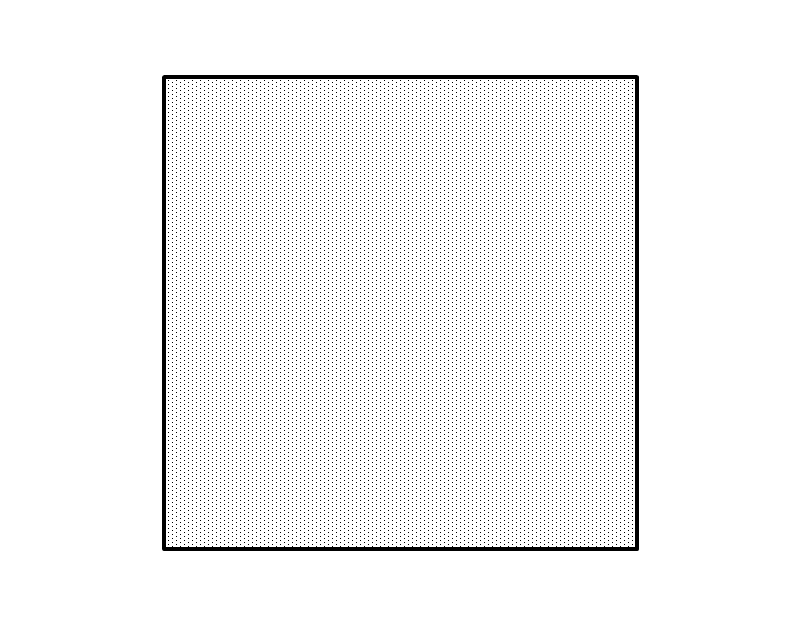
\includegraphics[scale=0.5]{szeliski_naiveEntree.png}}
		\subfigure[Spectre de l'image de sortie : repliement du spectre]{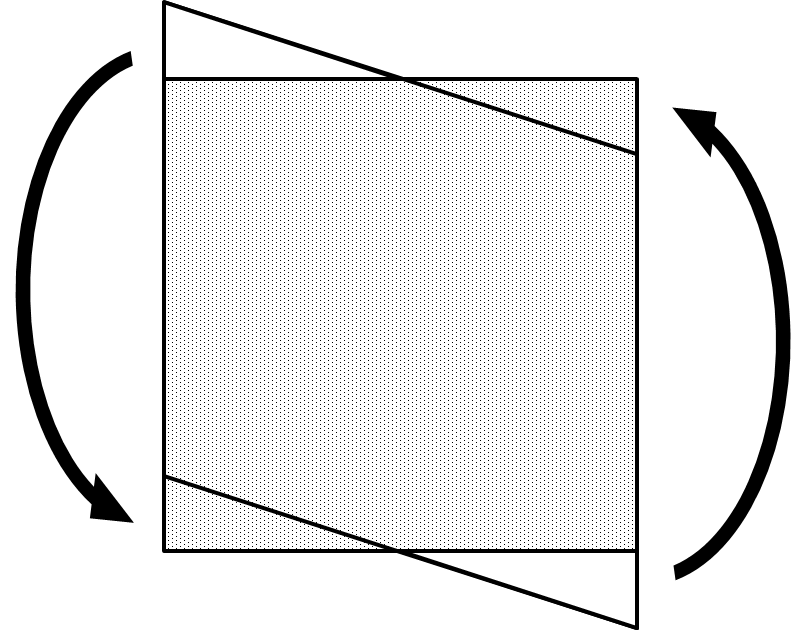
\includegraphics[scale=0.5]{szeliski_naiveSortie.png}}
		\caption{Effet d'un \emph{shear} sur le spectre de l'image (par la méthode naïve)}
		\label{szeliski_decompoNaive}
	\end{figure}
		
	\begin{figure}
		\centering
		\subfigure[Spectre de l'image d'entrée]{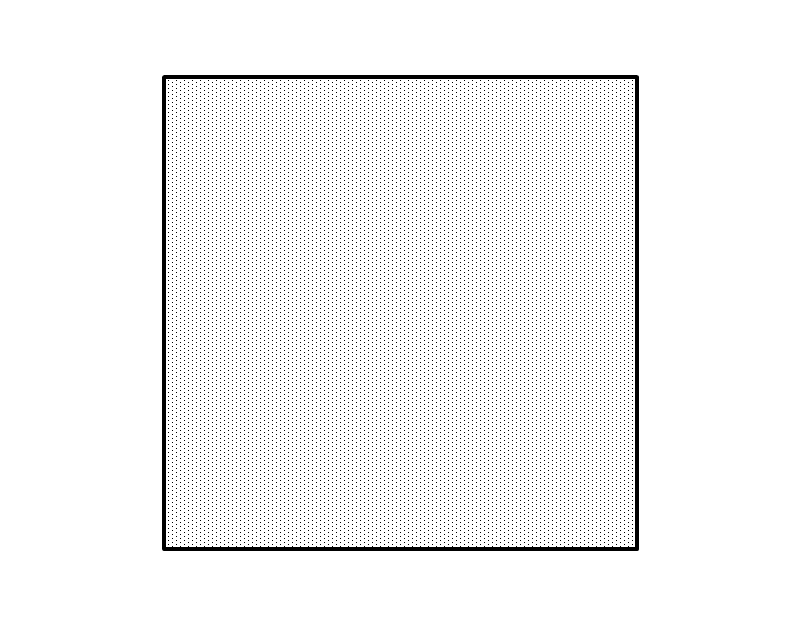
\includegraphics[scale=0.5]{szeliski_szeliskiEntree.png}}
		\subfigure[Spectre de l'image après sur-échantillonnage]{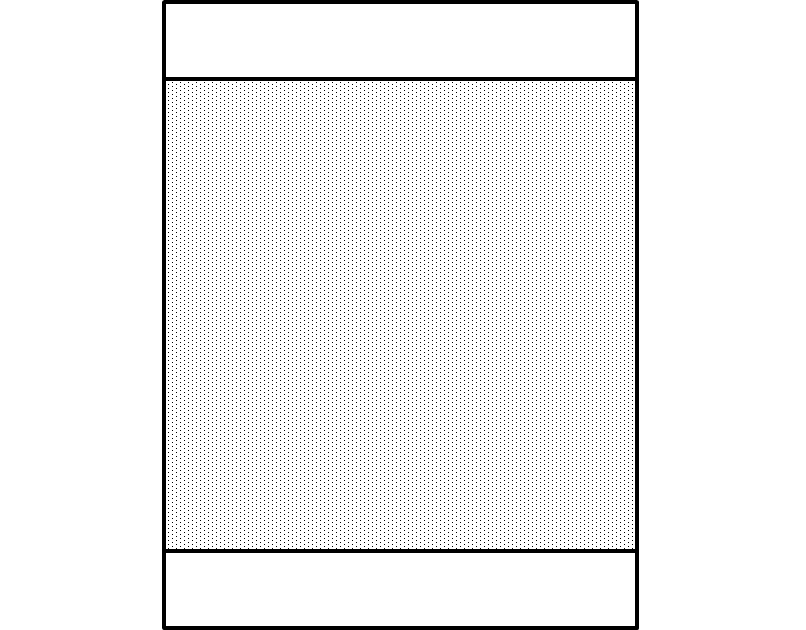
\includegraphics[scale=0.5]{szeliski_szeliskiSurechantillonnage.png}}
		\subfigure[Spectre de l'image après sur-échantillonnage et \emph{shear}]{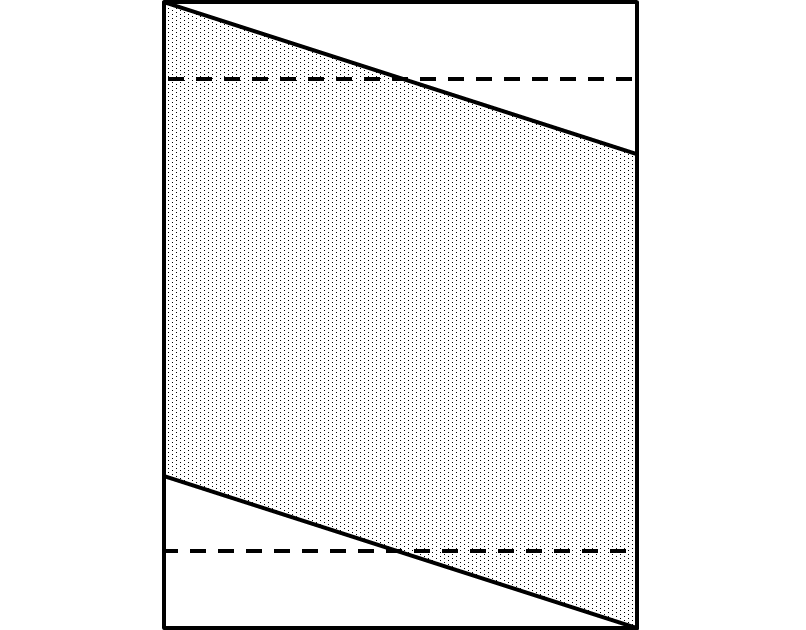
\includegraphics[scale=0.5]{szeliski_szeliskiShear.png}}
		\subfigure[Spectre de l'image de sortie (après sur-échantillonnage, \emph{shear} et sous-échantillonnage)]{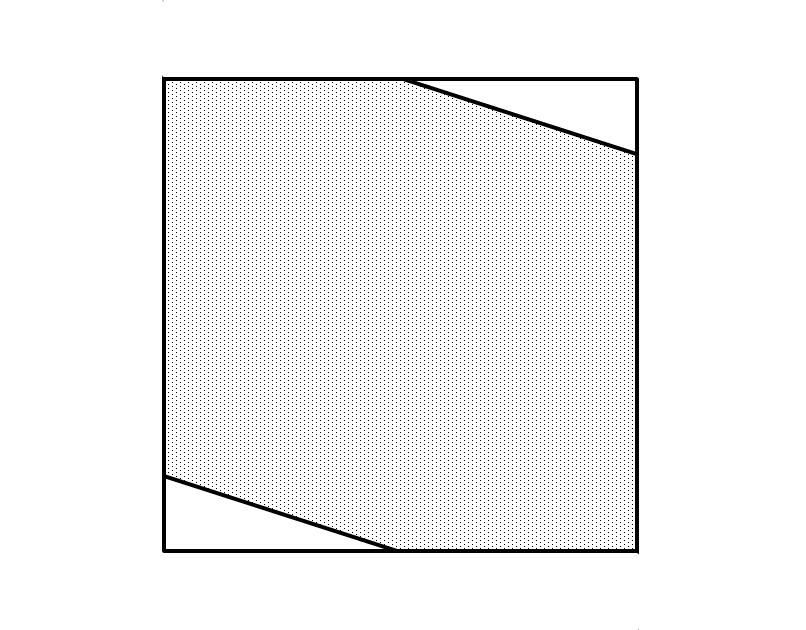
\includegraphics[scale=0.5]{szeliski_szeliskiSortie.png}}
		\caption{Effet d'un \emph{shear} sur le spectre de l'image (par le traitement multi-étapes). Mise en pratique figure \ref{experiments_decompoSzeliski_sinc}}
		\label{szeliski_decompoSzeliski}
	\end{figure}
	
	Ces trois opérations sont toutes des \emph{shears} (éventuellement réduit à une dilatation) et seront nommées $\mathcal R$ ; selon qu'elles modifient l'image verticalement (en laissant l'abscisse inchangée) ou horizontalement (en laissant l'ordonnée inchangée), on parlera de $\mathcal R_v$ ou de $\mathcal R_h$ . Ces opérations $\mathcal R$ sont réalisées par une convolution par un noyau d'interpolation, en l'occurrence une fonction de type \emph{raised cosine-weighted sinc}, pour pouvoir atténuer, voire supprimer, les fréquences au-delà d'un certain seuil.
	\[h : x \mapsto \sinc(\frac{x}{T})\frac{\cos(\frac{\pi\beta x}{T})}{1-\frac{4\beta^2x^2}{T^2}}\]
	La période $T$ est prise égale à 1 (taille d'un pixel).
	Le paramètre $\beta$, intitulé \emph{roll-off factor}, peut varier. En prenant $\beta$ autour de $0.36$ (paramètre utilisé pour la plupart des expériences en annexe), on peut considérer que le support de $h$ est compris dans $[-4,4]$, et donc réduire la convolution à une somme d'au plus 9 termes, tant que le support du filtre n'est pas modifié. En pratique, le support du filtre est adaptatif, et dépend d'un facteur de zoom $s$, d'où la formule de convolution par $h$ (ici convolution selon les abscisses) :
	\[ img_f[i][j] = \displaystyle{sum_k}h\left(\frac{a_0*i+a_1*j+t-k}{s}\right)img[k][j]\]
	où $img_f$ est l'image finale et $img$ l'image initiale (ici en une dimension).
	
	En multipliant par $s$ la taille du support du filtre (en appelant $h(\frac{x}{s})$ au lieu de $h(x)$, avec $s\geq 1$), on divise par $s$ la largeur de la bande passante de ce filtre. Cela permet, lors d'un sur-échantillonnage, d'avoir une protection contre l'\emph{aliasing}. Le coefficient $s$ dépend aussi des \emph{fréquences conservées maximales} $u_{max}$ et $v_{max}$ qui seront définies et expliquées plus loin.
	
	On est ainsi capable d'effectuer, en trois étapes $\mathcal R$ et sans \emph{aliasing}, tous les \emph{shears}. Or une affinité se décompose toujours en deux \emph{shears} (proposition \ref{propositionDecompositionAffinite}, on peut donc toujours traiter une affinité quelconque, et ce, sans \emph{aliasing}.

\begin{thm}
Le méthode multi-étapes \cite{szeliski2010high} empêche le repliement du spectre tout en conservant le maximum du spectre
\end{thm}
	Ce théorème est illustré figure \ref{szeliski_decompoSzeliski}  et vérifié en pratique figure \ref{experiments_decompoSzeliski_sinc}.
	
	Cette méthode semble donc décomposer une affinité en 6 opérations $\mathcal R$ (3 pour chacun des 2 \emph{shears}) ; en pratique, il est possible de réunir certains $\mathcal R$, s'ils sont dans la même direction. La décomposition peut alors se réduire à 4 opérations $\mathcal R$ : un sur-échantillonnage vertical, un \emph{shear} horizontal, un \emph{shear} vertical puis enfin un sous-échantillonnage horizontal.
	
\subsubsection{Étapes de l'algorithme}
	On détaille donc ici les étapes de l'algorithme de traitement d'une affinité par cette méthode multi-étape. Le pseudo-code correspondant est présent en annexe (algorithmes \ref{szeliski_rh}, \ref{szeliski_rv} et \ref{szeliski_affine}).
	
	On suppose avoir reçu en entrée une image à modifier et la matrice $A$ correspondant à l'affinité inverse de celle à effectuer : l'antécédent du point $(i,j)$ de l'image de sortie se situe donc en $A(i,j)$ sur l'image d'entrée.
	
	On notera
	\[A = \pmatrice{a_{00} & a_{01} & t_0\\ a_{10} & a_{11} & t_1}\]
	
	\paragraph{Éventuelle transposition}
		
		Les $\mathcal R$ peuvent, si l'affinité est par exemple une rotation d'angle $\frac{\pi}{2}$, compresser l'image sur peu de pixels puis tenter de la dilater ; cet effet est un \emph{bottleneck problem} déjà connu \cite{wolberg1990digital}.
		
		On effectue donc éventuellement une transposition (de l'image et de la matrice) pour éviter cet effet : en notant
		\[\hat a_{00} = \frac{a_{00}}{\sqrt{a_{00}^2+a_{11}^2}}\]
		\[\hat a_{01} = \frac{a_{01}}{\sqrt{a_{00}^2+a_{11}^2}}\]
		\[\hat a_{10} = \frac{a_{10}}{\sqrt{a_{10}^2+a_{11}^2}}\]
		\[\hat a_{11} = \frac{a_{11}}{\sqrt{a_{10}^2+a_{11}^2}}\]
		on transpose dans le cas où $|\hat a_{00}|+|\hat a_{11}|<|\hat a_{01}|+|\hat a_{10}|$.
		
	\paragraph{Décomposition de $A$}
		
		On introduit les fréquences conservées maximales $u_{max}$, $v_{max}$ : ce sont les fréquences, horizontales et verticales, au delà desquelles les fréquences seront effacées par l'application de $A$ ; elles sont donc définies dans le domaine de Fourier par la figure \ref{uMax_vMax}. Les fréquences au delà de $u_{max}$ horizontalement et de $v_{max}$ verticalement peuvent donc être filtrées, cela ne changera pas le spectre de sortie. Ces définitions se font après après avoir ramené le spectre sur le carré $[-1,1]^2$.
		
		\begin{figure}
		\centering
		\subfigure[Spectre de l'image d'entrée]{
\includegraphics[scale=0.5]{uMax_vMax_spectreEntree.png}}
		\subfigure[Spectre de l'image de sortie]{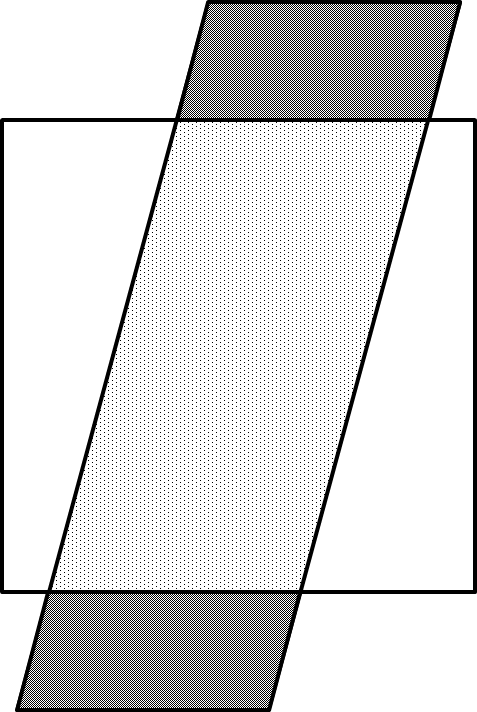
\includegraphics[scale=0.5]{uMax_vMax_spectreSortie.png}}
		\subfigure[Spectre de l'image d'entrée]{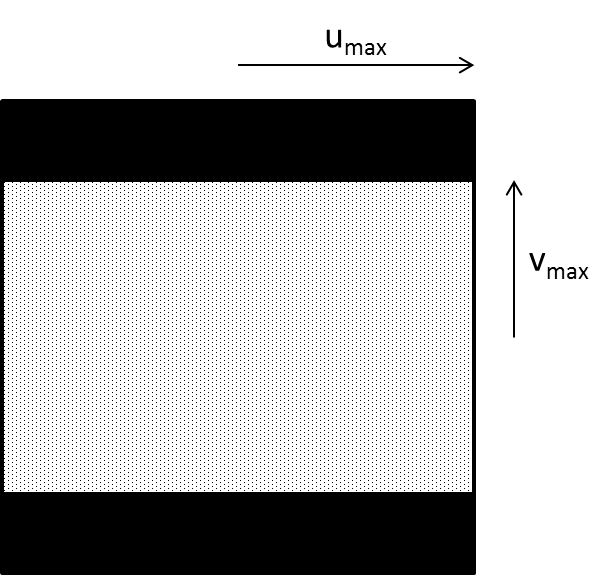
\includegraphics[scale=0.5]{uMax_vMax_spectreUtile.png}}
		\caption{Fréquences conservées par l'affinité. Les zones noires sont les fréquences qui ne seront pas conservées par l'application de l'affinité}
		\label{uMax_vMax}
		\end{figure}
		
		En pratique, $u_{max}$ et $v_{max}$ s'obtiennent en intersectant le spectre d'entrée (le carré $[-1,1]^2$) et l'image réciproque du carré $[-1,1]^2$ par $^t\!A$ (qui correspond à l'opération dans Fourier ; comme précédemment $A$ désigne l'inverse de l'affinité qu'on applique à l'image).
		
		À partir des coefficients de $A$ et des valeurs de $u_{max}$ et $v_{max}$, on peut en déduire les coefficients de sur-échantillonnage verticaux et horizontaux nécessaires \cite{szeliski2010high} :
		\[r_v \geq \max (1,|a_{01}|u_{max}+\min (1,|a_{11}|v_{max}))\]
		\[r_h \geq \max (1,|a_{10}/a_{11}|r_vv_{max}+\min (1,|b_0|u_{max}))\]
		Pour des raisons géométriques, on peut toujours réduire les sur-échantillonnages à $r_h \leq 3$ et $r_v \leq 3$. En effet, pour chacune des deux opérations unidirectionnelles (celles qui seront décomposées en trois $\mathcal R$), le $r_h$ (respectivement $r_v$) peut être réduit à 3, grâce au filtrage qui atténue les fréquences au delà de $u_{max}$ (respectivement $v_{max}$). La figure \ref{rvleq3} présente ce raisonnement géométrique pour une opération sur les colonnes (qui se traduit par une opération sur les lignes dans le domaine de Fourier).
		
		\begin{figure}
		\centering
		\subfigure[$r_v$ non majoré]{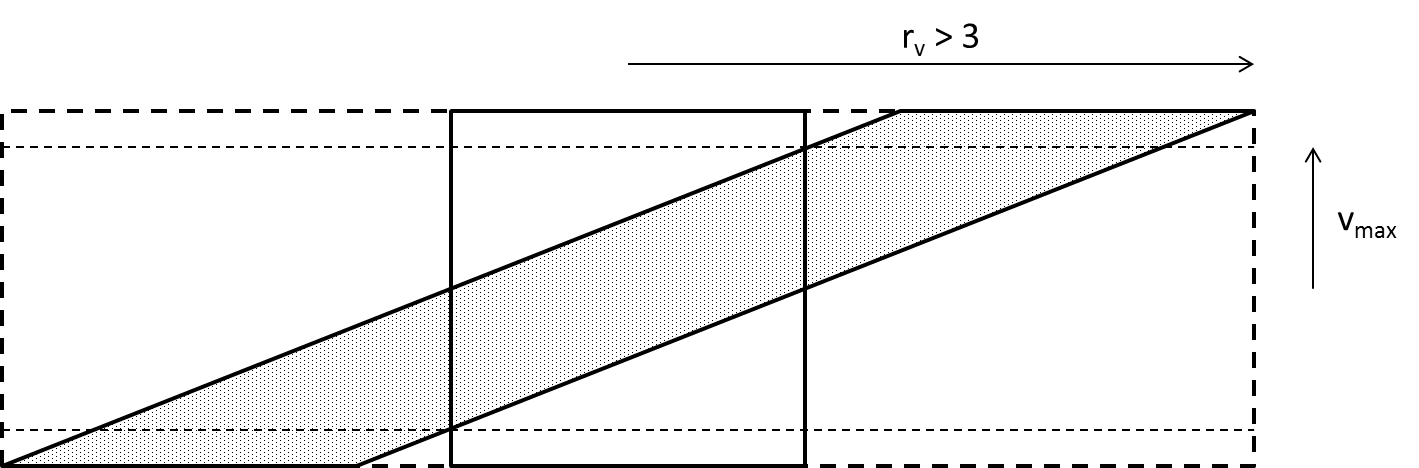
\includegraphics[width=120mm]{rvleq3_notrvleq3.png}}
		\subfigure[$r_v$ majoré par 3 ; on utilise le fait que les distances horizontales sont inchangées]{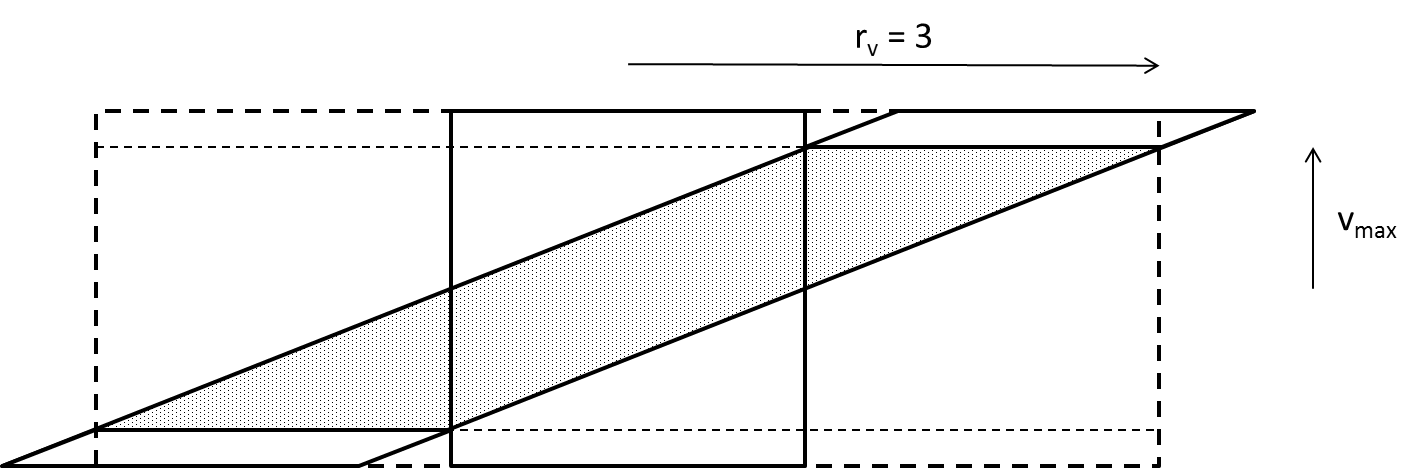
\includegraphics[width=120mm]{rvleq3_rveq3.png}}
		\caption{Réduction de $r_v$ jusqu'à $r_v \leq 3$. Au-delà de $v_{max}$, le filtre efface (atténue) les fréquences via le paramètre $s$ qui amincit la bande passante ; on peut alors réduire le $r_v$ nécessaire au non-repliement. $r_v$ est le quotient de la longueur du rectangle pointillé (spectre après sur-échantillonnage) par celle du carré (spectre initial)}
		\label{rvleq3}
		\end{figure}


		\begin{prop}
		\label{propositionDecompositionAffinite}
		Soit $A$ une affinité donnée sous forme projective : $A = \pmatrice{a_{00} & a_{01} & t_0\\ a_{10} & a_{11} & t_1\\ 0&0&1}$.
		
		$A$ se décompose de la manière suivante :
		\[
			A = 
			\pmatrice{1 & 0 & 0\\ 0 & \frac{a_{11}}{r_v} & 0\\ 0 & 0 & 1}
			\pmatrice{\frac{b_{0}}{r_h} & \frac{a_{01}}{r_v} & t_2\\ 0 & 1 & 0\\ 0 & 0 & 1}
			\pmatrice{1 & 0 & 0\\ \frac{a_{10}r_v}{a_{11}r_h} & r_v & \frac{t_1r_v}{a_{11}}\\ 0 & 0 & 1}
			\pmatrice{r_h & 0 & 0\\ 0 & 1 & 0\\ 0 & 0 & 1}
		\]
avec : $b_0 = a_{00} - \frac{a_{01}a_{10}}{a_{11}};$ et : $t_2 = t_0 - \frac{a_{01}t_1}{a_{11}}$.
\end{prop}
	\paragraph{Applications des $\mathcal R$}
		
		Il ne reste qu'à appliquer les quatre opérations $\mathcal R$.
		
		Pour chacune, on commence par stocker les différentes valeurs de $h(\frac{k+\varphi}{s})$ où
		\begin{itemize}
		\item $\varphi$ parcourt $2^b$ nombres rationnels de $[0,1]$ avec $b$ le nombre de bit de précision voulu
		\item $k$ parcourt les entiers tels que $\frac{k}{s}$ soit dans le support de $h$ ($h(x)$ étant presque nul quand $|x|$ est assez grand, on suppose $h$ à support compact)
		\end{itemize}
		On a ainsi accès rapidement à toutes les valeurs de $h$ qui peuvent être nécessaires à la convolution.
%shmuel
	\section{Décomposition géométrique d'une homographie}
		\label{decomp_geo_hom}
		\subsection{Décomposition d'une homographie en mouvement de caméra}
			Notre méthode de traitement des homographies repose sur la décomposition d'une homographie qui permet d'interpréter cette dernière en terme de mouvement de caméra. La partie ci-dessous présente cette décomposition.\\
\ssse{Mouvement de caméra :}
On étudie ici un cas a priori particulier d'homographie $h$   que l'on peut interpréter comme un mouvement de caméra ,on montrera par la suite que c'est en fait un cas général.\\
Nous modéliserons la situation en supposant que la scène filmée est bidimentionnelle, cela supposer que l'on est situé suffisamment loin de la scène observée, afin que les effets du relief soient négligeables. Le schéma de la figure suivante  illustre le modèle utilisé (figure \ref{shmdecomp}), les paramètres introduits sur ce schéma seront définitions et notations \ref{defpoint}.`\\
\begin{figure}[h!]

\centering
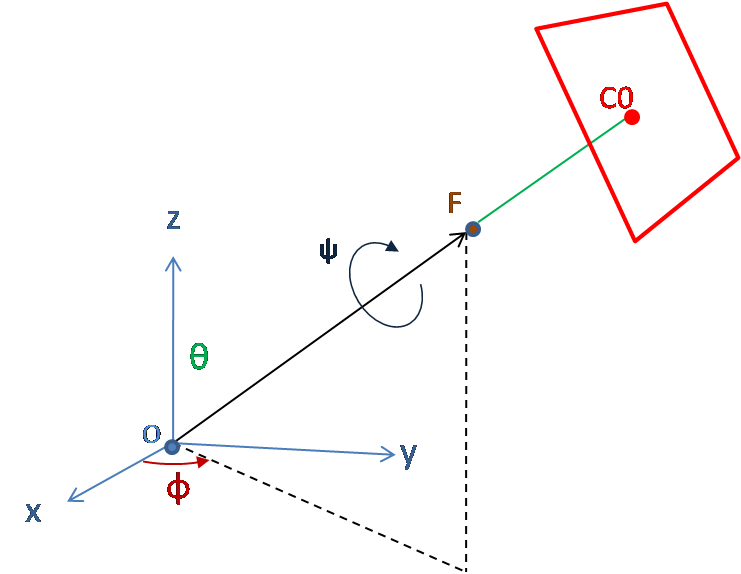
\includegraphics[width=10cm]{shema_decomp.png}
\caption{Illustration d'un mouvement de caméra $(X_v =0)$. $F$ représente le point focal de la caméra, le plan rouge est le plan image de la caméra.}
\label{shmdecomp}
\end{figure}
\begin{Def}
Une homographie unidirectionnelle est une application $h:\mathbb{R}^{2} \mapsto \mathbb{R}^{2}$ définit par 
\begin{equation*}
h(x,y)=\left ( \frac{ax+p}{rx+t} , \frac{cy+p}{rx+t} \right)
\end{equation*}
Où $a,p,c,q,r,t$ sont des réels 
\label{homo_uni_direc}
\end{Def}

\begin{defnot}
On se place dans l'espace $\mathbb{R}^{3}$,on le munit d'une base orthonormée directe $(x_0,y_0,z_0)$.\\
L'image de départ sera située dans le plan $P_{1}= \mathbb{R}^{2}\times \{0\}$.\\
On doit maintenant positionner notre caméra par rapport à l'image de départ (figure \ref{shmdecomp}).\\
\begin{itemize}
\item On note $F$ la position de l'objectif de la caméra, et $w$ le vecteur directeur unitaire de l'axe optique de la caméra. L'axe optique de la caméra est donc la droite passant par $F$ et dirigée par $w$.\\
\item On note $\delta$ la distance entre l'objectif et l'écran.\\
\item L'écran $P_{2}$ est alors le plan affine passant par $F+\delta w$ et perpendiculaire à l'axe optique de la caméra.
\begin{equation*}
P_{2}=\{Y\in \mathbb{R}^{3}|(Y-F-\delta w)\cdot w=0\}=\{Y\in \mathbb{R}^{3}|(Y-F)\cdot w=\delta\}
\end{equation*}
\item Si on se place dans le cas où le vecteur $w$ n'appartient pas à $P_{1}$, on peut alors définir $X_{v}$  le point de $P_{1}$ visé par la caméra, c'est-à-dire le point d'intersection entre l' axe optique et le plan $P_{1}$.On obtient alors
\begin{equation*}
X_{v}=F-\delta'w \text{ et }\delta'=\small{\left|\frac{F \cdot z_{0}}{w\cdot z_{0}} \right|}
\end{equation*}
\item La caméra peut aussi effectuer une rotation autour de son axe optique, que l'on appellera rotation propre et dont l'angle sera noté $\psi$.\\
\end{itemize}

On définit l'application $H$ qui à un point $X\in P_{1}$ lui associe sa projection homographique sur $P_{2}$. C'est-à-dire que le point $H(X)$ est le point d'intersection entre la droite $D_{X}$ passant par $X$ et $F$, et le plan $P_{2}$. Ce point n'est pas toujours défini, le domaine de définition de $H$ est $P_1$ privé d'une droite $D$ qui correspond à un angle mort de la caméra.
\begin{equation*}
D=\{X\in P_1 | (X-F) \cdot w=0\}
\end{equation*}
De même l'image de $H$ est $P_2 \setminus D'$ où $D'$ est appelé l'horizon du mouvement de \begin{equation*}
D'=\{ X\in P_2 | (X-F).z_0=0\}
\end{equation*}
Un mouvement de caméra est donc définit en fonction de $9$ paramètres, il n'y a d'unicité.
L'application $H$ est une bijection de $P_1 \setminus D$ dans $P_2 \setminus D'$ ,on peut remarquer que $H^{-1}$ est aussi un mouvement de caméra, de plus l'horizon de $H^{-1}$ est l'angle mort de $H$ et l'angle mort de $H^{-1}$ est l'horizon de $H$.\\
L'application $H$ est une version géométrique du mouvement de caméra. La formulation analytique du mouvement de est l'application $h:\mathbb{R}^{2} \setminus D \mapsto\mathbb{R}^{2}\setminus D'$, qui à un point $X\in P_1\setminus D$ de coordonnées $(x,y)$,  associe les coordonnées $h(x,y)$ du point $H(X)\in P_2 \setminus D'$ , dans le repère lié à la caméra.
On vera plus tard que $h$ est bien une homographie, c'est l'homographie associée au mouvement de caméra.\\
Le plan $P_1$ sera muni du repère orthonormé $(0,x_0,y_0)$, de même le plan affine $P_{2}$ peut être muni d'un repère orthonormé $(C,u,v)$ tel que la famille $(u,v,w)$ soit un base orthonormée directe de $\mathbb{R}^{3}$. La base $(u,v)$ est définit en fonction des  rotations effectuées par la caméra son expression sera précisée plus tard. Le point $C$ est un point arbitraire de $P_2$, on ne cherchera pas à vérifier la condition $C=C_0$ \\
Par abus de notation on note encore $D$ et $D'$ les droites de $\mathbb{R}^{2}$ lorsque l'on munit $P_1$ et $P_2$ des repères $(0,x_0,y_0)$ et $(C,u,v)$.  \\
On peut repérer le point $C$ par rapport au centre de l'écran $C_{0}$, c'est-à-dire la projection orthogonale de l'objectif sur l'écran : $C_{0}=Z+\delta w$ et $C=C_{0}+c_{u}u+c_{v}v$, on note $c=(c_u,c_v)$ et $x_v = (X_v \cdot x_0,X_v \cdot y_0)$.\\
\label{defpoint}
\end{defnot}
Dans la suite de cette section on fixe un jeux de paramètres $(\theta,\phi,\psi,\delta,\delta',c,Z)$ et on considère le mouvement de caméra $H$ associé à ces paramètres.\\
Dans cette partie on cherche à établir la décomposition suivante
\begin{prop}
$h$ est une homographie et si $H$ admet un point visé $X_v$ alors $h$ se factorise sous la forme
\begin{equation}
h = \tau_{c} \circ z_{\frac{\delta}{\delta'}}  \circ R_{\psi} \circ h_{\theta,\delta'} \circ R_{\phi} \circ \tau_{x_{v}}
\label{formul_decomp}
\end{equation}
Où $R_{\alpha}$ est la rotation d'angle $\alpha$,$z_\lambda$ est la dilatation de facteur $\lambda$, $\tau_y$ est  la translation du vecteur $-y$ et $h_{\theta,\delta'}$ est l'homographie unidirectionnelle (cf définition \ref{homo_uni_direc})
\begin{equation}
h_{\theta,\delta'}(x',y')=\left(\frac{-cos(\theta)x'}{1-\frac{sin(\theta)}{\delta'}x'} ,\frac{-y'}{1-\frac{sin(\theta)}{\delta'}x'}\right)
\label{mise_perspective}
\end{equation}
\label{prop_decomp}
\end{prop}
Ce résultat est intuitif et se comprend facilement grâce à la figure \ref{shmdecomp}, afin de le démontrer on commencera par établir deux lemmes

\begin{lem}Si le point visé $X_v$ existe alors
$\forall X \in P_1 \setminus D$
\begin{equation}
H(X)=Z+\delta w+\delta \frac{(X_v-X)-\left((X_v-X)\cdot w\right) w}{w\cdot (X_v-X)+\delta'}
\label{homo_form_geo}
\end{equation}
\end{lem}

\begin{proof}
On sait que $H(X)$ est le point d'intersection entre la droite $D_X$ passant par $X$ et $F$ , et le plan $P_2$.
Comme $D_{X}=\{X+t(F-X)|t\in\mathbb{R}\}$, si $H(X)$ existe alors 
\begin{equation*}
\exists t_{X},H(X)=X+t_{X}(F-X)
\end{equation*}
Comme $H(X)\in P_{2}$ alors
\begin{equation*}
(H(X)-F)\cdot w =\delta
\end{equation*}
Et donc 
\begin{equation*}
t_{X}=1+\frac{\delta}{w\cdot(F-X)}
\end{equation*}
 On en déduit que l'application $H$ est bien définie sur $P_{1}\setminus D$ et 
\begin{equation*}
H(X)=Z+\delta w+\delta \frac{(F-X)-\left((F-X)\cdot w\right) w}{w\cdot (F-X)}
\end{equation*}
Si le point visé $X_v$ existe alors  $F=X_v+\delta' w$ et donc
\begin{equation*}
H(X)=Z+\delta w+\delta \frac{(X_v-X)-\left((X_v-X)\cdot w\right) w}{w\cdot (X_v-X)+\delta'}
\end{equation*}
\end{proof}
Afin de simplifier les expressions dans les calculs qui suivent on défini la bijection $i$ 
\begin{equation*}
i:\mathbb{R}^{2}\rightarrow P_{1},~~~~~~i((x,y))=xx_{0}+yy_{0}
\end{equation*}

\begin{lem}Si le point visé $X_v$ existe alors $\forall X\in \mathbb{R}^{2} \setminus D$ 
\begin{equation}
h(X)=\left(\frac{\delta (X_{v}-i(X))\cdot u}{w \cdot (X_{v}-i(X)))+\delta'}-c_{u},\frac{\delta (X_{v}-i(X))\cdot v}{w \cdot (X_{v}-i(X))+\delta'} -c_{v} \right) 
\label{homo_form_analytique}
\end{equation}
\end{lem}
Ce lemme montre en particulier que $h$ est bien une homographie.
\begin{proof}
Par définition de $h$,les composantes de $h(X)$ sont les coordonnées de $H(i(X))$ dans le repère orthonormé $(C,u,v)$ de $P_2$ (cf notations et définitions \ref{defpoint}), on a donc $ \forall X\in \mathbb{R}^{2} \setminus D$
\begin{eqnarray*}
h(X) &=& ((H(i(X))-C)\cdot u, (H(i(X))-C)\cdot v)\\
     &=& ((H(i(X))-Z-\delta -c_u u -c_v v)\cdot u, (H(i(X))-Z-\delta -c_u u -c_v v)\cdot v)\\
     &=& ((H(i(X)-Z)\cdot u -c_u, (H(i(X))-Z)\cdot v - c_v)
\end{eqnarray*}
Grâce à la formule du lemme précédent (formule \ref{homo_form_geo}) on en déduit alors 
\begin{equation*}
h(X)=\left(\frac{\delta (X_{v}-i(X))\cdot u}{w \cdot (X_{v}-X))+\delta'}-c_{u},\frac{\delta (X_{v}-i(X))\cdot v}{w \cdot (X_{v}-i(X))+\delta'} -c_{v} \right) 
\end{equation*}
\end{proof}


On peut maintenant établir la formule de décomposition (formule \ref{formul_decomp} ) de la proposition \ref{prop_decomp}, les notations utilisées dans cette preuve ont été introduites au début de cette section (cf définitions et notations \ref{defpoint}).

\begin{proof}
On peut positionner le vecteur $w$ par rapport à la $(x_{0},y_{0},z_{0}) $ en introduisant deux angles, $\phi$ et $\theta$.

\begin{itemize}
\item la première rotation d'angle $\phi$ se fait autour de l'axe $(0,z_{0})$ ; on lui associe la base $(x_{1},y_{1},z_{1})$ où $z_{0}=z_{1}$.
\item la seconde rotation d'angle $\theta$ se fait autour de l'axe $(0,y_1)$ ; on lui associe la base $(x_{2},y_{2},z_{2})$ où $z_{2}=w$ et $y_{1}=y_{2}$.
\end{itemize}

\begin{figure}[h!]
\centering
\subfigure[rotation d'angle $\phi$]{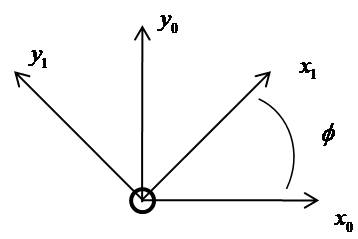
\includegraphics[width=5cm]{graphe1.jpg}}
\subfigure[rotation d'angle $\theta$]{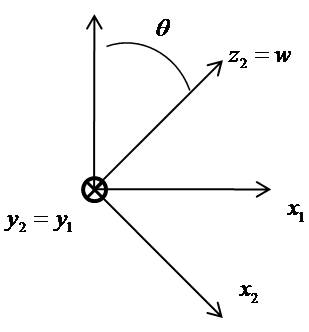
\includegraphics[width=5cm]{graphe2.jpg}}
\label{img_angles}
\end{figure}

Pour positionner la caméra, on doit définir sa rotation propre autour de son axe optique. Pour cela on définit l'angle $\psi$ (figure \ref{decompgeo_rotationPropre}).
\begin{figure}[h!]
\centering
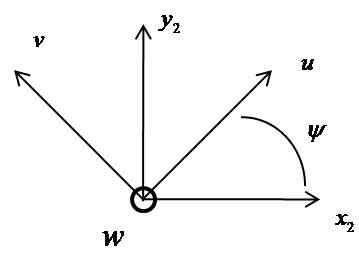
\includegraphics[width=5cm]{graphe3.jpg}
\caption{rotation propre}
\label{decompgeo_rotationPropre}
\end{figure}

On obtient alors (figure \ref{decompgeo_rotationPropre})
\begin{equation*}
u=\cos(\psi)x_{2}+\sin(\psi)y_{2} \text{ et } v=-\sin(\psi)x_{2}+\cos(\psi)y_{2}
\end{equation*}
Si on pose $R_{s}$ la rotation d'angle $s$ et $\tau_{y}$ la translation de vecteur $-y$, on obtient alors grâce au lemme précédent (formule \ref{homo_form_analytique})
\begin{eqnarray*}
(\tau_{c}^{-1} \circ h)(X) &=& \left(\frac{\delta (X_{v}-i(X))\cdot u }{w \cdot (X_{v}-i(X))+\delta'},\frac{\delta (X_{v}-i(X))\cdot y_{2}}{w \cdot (X_{v}-i(X))+\delta'}  \right) \\
                           &=& R_{\psi}\left(\frac{\delta (X_{v}-i(X))\cdot x_{2} }{w \cdot (X_{v}-i(X))+\delta'},\frac{\delta (X_{v}-i(X))\cdot y_{2}}{w \cdot (X_{v}-i(X))+\delta'}  \right) \\
\end{eqnarray*}
Comme  $X_{v}=i(x_{v})$ on obtient
\begin{equation*}
(R_{\psi}^{-1} \circ \tau_{c}^{-1}  \circ h)(X)=\delta \left(\frac{-i(\tau_{x_{v}} (X))\cdot x_{2} }{-w \cdot i(\tau_{x_{v}} (X))+\delta'},\frac{-i(\tau_{x_{v}} (X))\cdot y_{2}}{-w \cdot i(\tau_{x_{v}} (X))+\delta'}  \right) 
\end{equation*}

Comme $z_{2}=cos(\theta)z_{1}+sin(\theta)x_{1}$, $x_{2}=cos(\theta)x_{1}-sin(\theta)z_{1}$ (figure \ref{img_angles}) et $z_{1}\perp P_{1}$, on a

\begin{equation*}
(R_{\psi}^{-1} \circ \tau_{c}^{-1}  \circ h)(X)=\delta\left(\frac{-\cos(\theta)i(\tau_{x_{v}} (X))\cdot x_{1} }{\delta'-\frac{sin(\theta)}{\delta'}x_{1}\cdot i(\tau_{x_{v}}(X))}, \frac{-i(\tau_{x_{v}} (X))\cdot y_{1}}{\delta'-\frac{sin(\theta)}{\delta'}x_{1}\cdot i(\tau_{x_{v}}(X))}  \right) 
\end{equation*}

En définissant $h_{\theta,\delta'}$ par

\begin{equation*}
h_{\theta,\delta'}(x',y')=\left(\frac{-cos(\theta)x'}{1-\frac{sin(\theta)}{\delta'}x'} ,\frac{-y'}{1-\frac{sin(\theta)}{\delta'}x'}\right)
\end{equation*}

Alors 

\begin{equation*}
(R_{\psi}^{-1} \circ \tau_{c}^{-1} \circ h)(X)= \frac{\delta}{\delta'}h_{\theta,\delta'}\left ( i(\tau_{x_{v}}(X)) \cdot x_{1}, i(\tau_{x_{v}}(X)) \cdot y_{1}\right)
\end{equation*}

Comme $x_{1}=\cos(\phi)x_{0}+\sin(\phi)y_{0}$ et $y_{1}=-\sin(\phi)x_{0}+\cos(\phi)y_{0}$ (figure \ref{img_angles}), alors

\begin{eqnarray*}
(R_{\psi}^{-1} \circ \tau_{c}^{-1} \circ h)(X) &=& \frac{\delta}{\delta'}h_{\theta,\delta'}\left ( R_{\phi}(i(\tau_{x_{v}}(X)) \cdot x_{0}, i(\tau_{x_{v}}(X)) \cdot y_{0})\right)\\
                                               &=&\frac{\delta}{\delta'} (h_{\theta,\delta'}\circ R_{\phi} \circ \tau_{x_{v}})(X)
\end{eqnarray*}

Si on définit les dilatations $z_{\lambda}:X\rightarrow \lambda X$, alors on obtient la formule générale pour les mouvements de caméra

\begin{equation*}
h = \tau_{c} \circ z_{\frac{\delta}{\delta'}}  \circ R_{\psi} \circ h_{\theta,\delta'} \circ R_{\phi} \circ \tau_{x_{v}}
\end{equation*}

\end{proof}
On verra plus tard qu'une homographie admet plusieurs décompositions il n'y a pas unicité des paramètres $(\theta,\phi,\psi,\delta,\delta',c,x_v)$
\begin{Remaffin}
Une homographie associée à un mouvement de caméra est une application affine si et seulement si $\theta=0$ dans ce cas la on obtient  
\begin{equation*}
h=z_{-\frac{\delta}{\delta'}} \circ \tau_c \circ R_{\phi+\psi} \circ \tau_{x_{v}}
=\tau' \circ z_{-\frac{\delta}{\delta'}} \circ  R_{\phi+\psi}
\end{equation*}
Toutes les applications affines ne sont donc pas des mouvements de caméra.\\
On peut cependant les voir comme un cas limite, fixons le rapport  $k=\frac{\delta}{\delta'}$ si l'on fait tendre $\delta'$ et $\delta$ vers $+\infty$ la fonction $h_{\theta,\delta'}$ tend vers une limite $h_{\theta,\infty}$ définie par
\begin{equation*}
h_{\theta,\infty}=(x,y)=(-\cos(\theta)x,-y)
\end{equation*}
Physiquement cela revient à s'éloigner de la scène en tout  en augmentant la focale afin de ne pas modifier la taille de l'image en sortie de l'appareil.\\
Si on pose $h_\infty = z_{-\frac{\delta}{\delta'}} \circ \tau_c \circ R_{\phi} \circ h_{\theta,\infty} \circ R_{\psi} \circ \tau_{x_{v}}$ la partie linéraire de $h_{\infty}$ peut être représentée par la matrice $2\times2$

\begin{equation*}
R_{\psi} \cdot 
\begin{pmatrix}
-k\cos(\theta)&0\\
0&-k
\end{pmatrix}
\cdot R_{\phi}
\end{equation*}

Si  $M$ est une matrice $2\times 2$  inverssible on à alors le lemme suivant qui provient de la décomposition en valeurs singulières \\
\begin{lem}
Il existe deux matrices de rotations $R_1$ et $R_2$  et une matrice diagonale $D$ telles que $M = R_1 \cdot D \cdot R_2$.
\end{lem}
Grâce à ce lemme on peut en déduire que pour toute application affine bijective $A$ il existe un changement de caméra $h$ tel que $h_\infty = A$, on peut deplus supposer que $h$ 
ne translate pas en sortie.
\end{Remaffin}


\subsubsection{Application à la décomposition des homographies :}
Le but de cette partie est généraliser cette décomposition à toutes les homographies qui ne sont pas des applications affines.
\begin{prop}
Toute homographie est un mouvement de caméra avec un point visé ou une application affine. Dans le premier cas, la décomposition \ref{formul_decomp} n'est pas unique et possède un degré de liberté..
\label{thepropdecomp}
\end{prop}
\paragraph{Résultats généraux sur les homographies :}
 On rappelle ici les notions sur les homographies qui seront utiles dans la suite. Le lien entre les homographies et les espaces projectifs ne sera pas étudié. On rappelle que dans ce document, une homographie $h$ est une application bijective de la forme :
	\[h:(x,y)\mapsto \left(\frac{ax+by+p}{rx+sy+t},\frac{cx+dy+q}{rx+sy+t}\right)\]
(l'ensemble d'arrivée est $\mathbb R^2$ privé d'une droite).

Les applications affines sont un cas particulier d'homographie ; si une homographie n'est pas une application affine alors elle est définie sur le plan privé d'une droite.

L'ensemble des homographies a une structure de groupe pour la loi de composition.

On peut  associer à l'homographie $h$ la matrice $H$ définies par
  
\begin{equation*}
	H=\begin{pmatrix}
	a&b&p\\c&d&q\\r&s&t
	\end{pmatrix}
\end{equation*}
Cette matrice est inversible car $h$ est inversible, elle n'est pas unique car la matrice $\lambda H$ définit la même homographie pour $\lambda \in \mathbb{R}_+$.

Cette notation rend compatible le produit matriciel et la composition des homographies. On obtient un morphisme de groupe de $GL_{3}(\mathbb{R})$ dans le groupe des homographies du plan. Ce morphisme n'est pas injectif, la matrice d'une homographie est définie à proportionnalité près mais il se quotiente à travers $SL_{3}(\mathbb{R})$ en un isomorphisme.

Dans la suite on notera $\sim$ la relation d'équivalence  sur $GL_{3}(\mathbb{R})$ définie par $A\sim B \iff \exists \lambda\in \mathbb{R}^{*} , A=\lambda B$, c'est-à-dire si, et seulement si, $A$ et $B$ définissent la même homographie.

\paragraph{Décomposition matricielle :}
Le but de cette partie est d'établir la proposition \ref{thepropdecomp}
%la ref n'apparait pas bien
\begin{proof}
On fixe $h$ une homographie et $H$ une matrice qui lui est associée. On conserve ici les notations de la partie précédente, on suppose sans perte de généralité que $\det (H)=1$. On suppose de plus que $h$ peut s'écrire sous la forme $\ref{formul_decomp}$, on cherche à montrer que cette hypothèse n'impose aucune condition supplémentaire sur la matrice $H$, en déterminant les paramètres intervenants dans la décomposition en fonction des coefficients de $H$ .

On a la formule de décomposition :

\begin{equation*}
h= \tau_{c} \circ z_{\frac{\delta}{\delta'}}\circ R_{\psi} \circ h_{\theta,\delta'} \circ R_{\phi} \circ \tau_{x_{v}}
\end{equation*}
Chacune de ces transformations est une homographie, on peut donc réécrire cette relation en utilisant des matrices. On obtient 
 \begin{equation*}
H\sim T_{c} Z_{\frac{\delta}{\delta'}}  R_{\psi}  H_{\theta,\delta'} R_{\phi}  T_{x_{v}}
\end{equation*}
avec
\begin{equation*}
R_{\alpha}=\begin{pmatrix}
\cos(\alpha)&\sin(\alpha)&0\\-\sin(\alpha)&cos(\alpha)&0\\0&0&1
\end{pmatrix}
, H_{\theta,\delta'}=\begin{pmatrix}
-\cos(\theta)&0&0\\0&-1&0\\-\frac{\sin(\theta)}{\delta'}&0&1
\end{pmatrix},
\end{equation*}
\begin{equation*}
Z_{\lambda}=\begin{pmatrix}
\lambda&0&0\\0&\lambda&0\\0&0&1
\end{pmatrix}
\text{ et } T_{X_{v}}=\begin{pmatrix}
1&0&-x_{v}\\0&1&-y_{v}\\0&0&1
\end{pmatrix}
\end{equation*}
 On cherche dans un premier temps à déterminer les translations. Soient $X_1 = (x_1 , y_1 )$ et $X_2 = (x_2 , y_2 )$ deux vecteurs que l'on suppose tel que la matrice $H_t$ définie par $H_t = T_{-X_2}  \cdot H \cdot T_{X_1}$ admette une décomposition de la forme  $H_t=R_{\psi} \cdot H_{\theta,\delta} \cdot R_{\phi}$.
 
 On notera
 \begin{equation*}
 H^{-1}=\begin{pmatrix} \hat a&\hat b&\hat p\\ \hat c&\hat d&\hat q\\ \hat r&\hat s&\hat t \end{pmatrix}
 \end{equation*}
 Par un calcul on obtient que la matrice $R_{\psi} \cdot H_{\theta,\delta} \cdot R_{\phi}$ est égale à : 
  \begin{equation*}
\begin{pmatrix}
 -\frac{\delta}{\delta'}\cos(\psi)\cos(\theta)\cos(\phi)+\frac{\delta}{\delta'}\sin(psi)\sin(\phi)& -\frac{\delta}{\delta'}\cos(\psi)\cos(\theta)\sin(\phi)-\frac{\delta}{\delta'}\sin(\psi)\cos(\phi)&0\\
  \frac{\delta}{\delta'}\sin(\psi)\cos(\theta)\cos(\phi)+\frac{\delta}{\delta'}\cos(\psi)\sin(\phi)& \frac{\delta}{\delta'}\sin(\psi)\cos(\theta)\sin(\phi)-\frac{\delta}{\delta'}\cos(\psi)\cos(\phi)&0\\ -\frac{\sin(\theta)}{\delta'}\cos(\phi)&-\frac{\sin(\theta)}{\delta'}\sin(\phi)& 1
 \end{pmatrix}
 \end{equation*}
 On a de plus 
 \begin{equation*}
 H_t=\begin{pmatrix}
 a-x_2 r&b-x_2 s& a x_1 + b y_1 + p -x_2 (r x_1 +s y_1 +t)\\
  c-y_2 r&d-y_2 s& c x_1 + d y_1 + q -y_2 (r x_1 +s y_1 +t)\\
  r & s & r x_1 + s y_1 +t
 \end{pmatrix}
 \end{equation*}
 On a donc l'équivalence 
 \begin{equation*}
 (H_t)_{1,3}=(H_t)_{2,3}=0 \iff (x_2,y_2)=h(x_1,y_1) \iff (x_1,y_1)=h^{-1}(x_2,y_2)
 \end{equation*}
 On pose $(x_1,y_1)=h^{-1}(x_2,y_2)$ car les calculs intermédiaires sont moins fastidieux, on suppose $(x_2,y_2)$ tels que $\hat r x_2 +\hat s y_2 + \hat t \ne 0$.\\
On obtient alors
\begin{equation*}
H_t
  \sim 
  \begin{pmatrix}
 (a-x_2 r)(\hat r x_2 + \hat s y_2 +\hat t)&(b-x_2 s)(\hat r x_2 + \hat s y_2 +\hat t)& 0\\
  (c-y_2 r)(\hat r x_2 + \hat s y_2 +\hat t)&(d-y_2 s)(\hat r x_2 + \hat s y_2 +\hat t)& 0\\
  r(\hat r x_2 + \hat s y_2 +\hat t) & s(\hat r x_2 + \hat s y_2 +\hat t) &1
  \end{pmatrix} 
\end{equation*}
On obtient alors 
 \begin{equation*}
 -\frac{\sin(\theta)}{\delta'}\cos(\phi)=r(\hat r x_2 + \hat s y_2 +\hat t)\text{ et } -\frac{\sin(\theta)}{\delta'}\sin(\phi)=s(\hat r x_2 + \hat s y_2 +\hat t)
 \end{equation*}
 On sait que $r^{2}+s^{2}=0$ si et seulement si l'homographie associée à H est une affinité. Ce cas ci sera traité de façon indépendante, on suppose ici que l'homographie $h$ n'est pas une affinité. On peut donc écrire :
 \begin{eqnarray*}
 \cos(\psi) &=& \sgn\left(-\frac{\sin(\theta)}{ \delta'}\right)\sgn(\hat r x_2 + \hat s y_2 +\hat t)\frac{r}{\sqrt{r^{2}+s^{2}}}\\
 \sin(\psi) &=& \sgn\left(-\frac{\sin(\theta)}{ \delta'}\right)\sgn(\hat r x_2 + \hat s y_2 +\hat t)\frac{s}{\sqrt{r^{2}+s^{2}}}
 \end{eqnarray*}
 On peut se restreindre au cas $\frac{\sin(\theta)}{\delta'}>0$ :\\
 \begin{itemize}
 \item En effet si $\frac{\sin(\theta)}{\delta'}<0$ on obtient alors
 \begin{equation*}
 R_{\psi} \cdot H_{\theta,\delta'} \cdot R_{\phi}=R_{\psi} \cdot Z_{-1}\cdot H_{\theta,-\delta'}\cdot Z_{-1} \cdot R_{\phi}= R_{\psi+\pi} \cdot H_{\theta,-\delta'}\cdot R_{\phi+\pi}
 \end{equation*}
 et on a $-\frac{\sin(\theta)}{\delta'}>0$.\\
 \end{itemize}


 On obtient alors 
 \begin{equation*}
 \cos( \phi )= -\sgn(\hat r x_2 +\hat s y_2 +\hat t) \frac{r}{\sqrt{r^2 + s^2}} \text{ et } \sin( \phi )= -\sgn(\hat r x_2 +\hat s y_2 +\hat t) \frac{s}{\sqrt{r^2 + s^2}}
 \end{equation*}
 Comme 
 \begin{equation*}
H_t \cdot R_{\phi}^{-1} \sim
 \begin{pmatrix}
 -|\hat r x_2 +\hat s y_2 +\hat t|\frac{(ar+sb)-(r^2 + s^2)x_2}{\sqrt{r^2 + s^2}}&-|\hat r x_2 +\hat s y_2 +\hat t|\frac{\hat s}{\sqrt{r^2 + s^2}}&0\\
 -|\hat r x_2 +\hat s y_2 +\hat t|\frac{(cr+sd)-(r^2 + s^2)y_2}{\sqrt{r^2 + s^2}}&|\hat r x_2 +\hat s y_2 +\hat t|\frac{r}{\sqrt{r^2 + s^2}}&0\\
 -|\hat r x_2 +\hat s y_2 +\hat t|\sqrt{r^2 + s^2}&0&1
 \end{pmatrix}
 \end{equation*}
 Et d'un autre côté 
 \begin{equation*}
R_{\psi} \cdot H_{\theta,\delta}  \sim 
 \begin{pmatrix}
 -\frac{\delta}{\delta'}\cos(\psi)\cos(\theta)&
-\frac{\delta}{\delta'}\sin(\psi)&
0\\
\frac{\delta}{\delta'}\sin(\psi)\cos(\theta)&
-\frac{\delta}{\delta'}\cos(\psi)&
0\\
-\frac{\sin(\theta)}{\delta'}&
0&
1
 \end{pmatrix}
 \end{equation*}
Comme $h$ n'est pas une affinité on a $\hat r^2 + \hat s^2 \ne 0$ 
 \begin{equation*}
  \cos( \psi ) =- \sgn(\frac{\delta}{\delta'})\frac{\hat r}{\sqrt{\hat r^2 + \hat s^2}}\text{ et } \sin( \psi ) = \sgn(\frac{\delta}{\delta'})\frac{\hat s}{\sqrt{\hat r^2 + \hat s^2}}
 \end{equation*}
On peut se restreindre au cas $\frac{\delta}{\delta'}>0$ :\\
\begin{itemize}
\item En effet si $\frac{\delta}{\delta'}<0$ on obtient alors $Z_{\frac{\delta}{\delta'}} \cdot R_{\psi}=Z_{\left|\frac{\delta}{\delta'}\right|}\cdot Z_{-1} \cdot R_{\psi}=Z_{\left|\frac{\delta}{\delta'}\right|}\cdot R_{\pi} \cdot R_{\psi}=Z_{\left|\frac{\delta}{\delta'}\right|}\cdot R_{\psi+\pi}$.
\end{itemize}
Et donc 
 \begin{equation*}
  \cos( \psi ) =- \frac{\hat r}{\sqrt{\hat r^2 + \hat s^2}} \text{ et } \sin( \psi ) = \frac{\hat s}{\sqrt{\hat r^2 + \hat s^2}}
 \end{equation*}



 On obtient alors 
\begin{equation*}
R_{\psi}^{-1} \cdot H_t \cdot R_{\phi}^{-1} \sim 
 \begin{pmatrix}
 -|\hat r x_2 +\hat s y_2 +\hat t|(\hat r x_2 +\hat s y_2 +\hat t)\sqrt{\frac{r^2 + s^2}{\hat r^2 + \hat s^2}}&0&0\\
 |\hat r x_2 +\hat s y_2 +\hat t|\frac{\Delta_H(x_2 , y_2)}{\sqrt{r^2 + s^2}\sqrt{\hat r^2 + \hat s^2}}&-|\hat r x_2 +\hat s y_2 +\hat t|\sqrt{\frac{\hat r^2 + \hat s^2}{r^2 + s^2}}&0\\
 -|\hat r x_2 +\hat s y_2 +\hat t|\sqrt{r^2 + s^2}&0&1
 \end{pmatrix}
\end{equation*}
Où l'on a posé 
\begin{equation*}
\Delta_H(x_2 , y_2 ) =\hat r ((rc+sd)-(r^2 + s^2)y_2) - \hat s ((ar+sb)-(r^2 + s^2 )x_2)
\end{equation*}
Les solutions de $\Delta_H(x_2 , y_2 )=0$ sont
\[ \left\lbrace \left( x_2=\frac{ar+sb+ \hat r \lambda}{r^2 +s^2}, y_2=\frac{cr+sd+\hat s \lambda}{r^2 +s^2}\right), \lambda \in \mathbb R \right\rbrace\]
On a dans ce cas
\begin{equation*}
\hat r x_2 +\hat s y_2 +\hat t = \frac{\hat r^2 +\hat s^2}{r^2 + s^2} \lambda
\end{equation*}
Le paramètre $\lambda$ doit donc être pris différent de zéro car 
\begin{equation*}
R_{\psi}^{-1} \cdot H_t \cdot R_{\phi}^{-1} \sim 
 \begin{pmatrix}
 -| \lambda | \lambda \sqrt{\frac{\hat r^2 + \hat s^2}{s^2 + r^2}}^{3}&0&0\\
0&-| \lambda | \sqrt{\frac{\hat r^2 + \hat s^2}{r^2 + s^2}}^{3}&0\\
 -|\lambda|\frac{\hat r^2 + \hat s^2}{\sqrt{r^2 + s^2}}&0&1
 \end{pmatrix}
\end{equation*}
 
 
 On peut poser 
 \begin{equation*}
 \frac{\delta}{\delta'}=|\lambda|\sqrt{\frac{\hat r^2 + \hat s^2}{r^2 + s^2}}^{3}
 \end{equation*}
On obtient finalement
\begin{equation*}
Z_{\frac{\delta}{\delta'}}^{-1} \cdot R_{\psi}^{-1} \cdot H_t \cdot R_{\phi}^{-1} \sim 
 \begin{pmatrix}
 -\lambda&0&0\\
0&-1&0\\
 -|\lambda|\frac{\hat r^2 + \hat s^2}{\sqrt{r^2 + s^2}}&0&1
 \end{pmatrix}
 \end{equation*}
 Cette matrice doit être de la forme $H_{\theta,\delta'}$. Pour qu'elle le soit, on doit avoir 
 \begin{equation*}
  \lambda^2 + \lambda^2 \delta'^2 \frac{(\hat r^2 + \hat s^2)^2}{r^2 + s^2}=1
 \end{equation*}
 C'est-à-dire
 \begin{equation*}
  \delta'^2 = (r^2 + s^2) \frac{1-\lambda^2}{\lambda^2 (\hat r^2+\hat s^2)^2}
 \end{equation*}
\end{proof}
 %\paragraph{Synthèse et optimisation :}
 %On a montré dans la section précédente que toute homographie qui n'est pas une application affine est un mouvement de caméra. On a de plus que pour tout $\lambda \in ]0,1[$ %pas certain que c'est ce que tu veux dire
 %\begin{equation*}
%x_2=\frac{ar+sb+\hat r \lambda}{r^2 +s^2}, y_2=\frac{cr+sd+\hat s \lambda}{r^2 +s^2}, (x_1 , y_1) = h^{-1}(x_{2},y_{2})
%\end{equation*}
 %\begin{equation*}
 %\cos( \phi )= - \frac{r}{\sqrt{r^2 + s^2}},  \sin( \phi )= - \frac{s}{\sqrt{r^2 + s^2}}, \cos( \psi ) =- \frac{\hat r}{\sqrt{\hat r^2 + \hat s^2}},  \sin( \psi ) = \frac{\hat s}{\sqrt{\hat r^2 + \hat s^2}}
 %\end{equation*}
 %\begin{equation*}
 %\frac{\delta}{\delta'}=|\lambda|\sqrt{\frac{\hat r^2 + \hat s^2}{r^2 + s^2}}^{3}, \cos(\theta)=\lambda, \sin(\theta)=\sqrt{1-\lambda^2}, \delta'=  \frac{\sqrt{(r^2 + s^2)(1-\lambda^2)}}{|\lambda| (\hat r^2+\hat s^2)}
 %\end{equation*}
 %Le degré de liberté correspond à une translation en sortie dans une direction perpendiculaire à l'horizon de $H^{-1}$.\\
 %Une décomposition plus générale autorise $\lambda \in \mathbb{\hat r}^{*}$.
%

 \paragraph{Synthèse et utilisation :}
  On a donc montré que toute homographie (autre qu'une affinité) peut s'identifier à un mouvement de caméra. Plus précisément, pour tout $\lambda \in ]0,1[$,

  \begin{equation*}
H \sim T_{c} Z_{\frac{\delta}{\delta'}}  R_{\psi}  H_{\theta,\delta'} R_{\phi}  T_{x_{v}}
  \end{equation*}
  avec $T_c$ translation de vecteur $(x_2,y_2)$, $T_{x_v}$ translation envoyant $(0,0)$ sur le point visé $X_v$, et
 \begin{equation*}
x_2=\frac{ar+sb+\hat r \lambda}{r^2 +s^2}, y_2=\frac{cr+sd+\hat s \lambda}{r^2 +s^2}, (x_1 , y_1) = h^{-1}(x_{2},y_{2})
  \end{equation*}
 \begin{equation*}
 \cos( \phi )= - \frac{r}{\sqrt{r^2 + s^2}}, \sin( \phi )= - \frac{s}{\sqrt{r^2 + s^2}},\cos( \psi ) =- \frac{\hat r}{\sqrt{\hat r^2 + \hat s^2}}, \sin( \psi ) = \frac{\hat s}{\sqrt{\hat r^2 + \hat s^2}}
 \end{equation*}
 \begin{equation*}
 \frac{\delta}{\delta'}=|\lambda|\sqrt{\frac{\hat r^2 + \hat s^2}{r^2 + s^2}}^{3}, \cos(\theta)=\lambda, \sin(\theta)=\sqrt{1-\lambda^2}, \delta'=  \frac{\sqrt{(r^2 + s^2)(1-\lambda^2)}}{|\lambda| (\hat r^2+\hat s^2)}
 \end{equation*}
 Le degré de liberté $\lambda$ correspond à une translation en sortie dans une direction perpendiculaire à l'horizon de $H^{-1}$.
 
 On peut commuter $Z_{\frac{\delta}{\delta'}}$ et $R_{\psi}$, et introduire une translation $T'$ telle que $R_{\phi}  T_{x_{v}} = T' R_\phi$. On arrive donc à une décomposition
   \begin{equation*}
H \sim T_{c} R_{\psi}  \tilde H R_{\phi}
  \end{equation*}
  Les affinités $T_{c} R_{\psi}$ et $R_{\phi}$ sont des isométries, et même principalement des rotations (la translation pouvant être prise en compte en considérant qu'on change l'endroit du plan traité). Il existe donc déjà des manières efficaces de les traiter (étudiée en \ref{YaroSzeli}).
  
  L'homographie $\tilde H$ est une homographie de la forme
  \[\tilde H = \pmatrice{*&0&*\\ 0&*&*\\ *&0&*}\]
  qui est une forme particulière permettant d'être plus facilement qu'une homographie quelconque (voir \ref{HomoboxRipmap}).
  
 Formellement, on peut s'autoriser $\lambda \in \mathbb R^*$ ; la décomposition matricielle reste alors correcte, mais elle perd son interprétation géométrique ($\lambda$ ne peut plus être identifié à un cosinus). De plus, on peut prendre $\phi + \pi$ au lieu de $\phi$ (de même pour $\psi$), car cela aura uniquement pour effet de multiplier certains coefficients de $\tilde H$ par $-1$.
 
 On en déduit donc un traitement d'une homographie générale, non affine, en passant par deux rotations-translations et une homographie particulière, correspondant à l'algorithme \ref{pseudoCodeDecompo}. Le traitement des affinités et des homographies correspond aux deux prochaines parties.
		
	\begin{figure}
		\centering
		\subfigure[Vue de départ]{
		{
\includegraphics[width=60mm]{vue_fps_identity.jpg}}
		{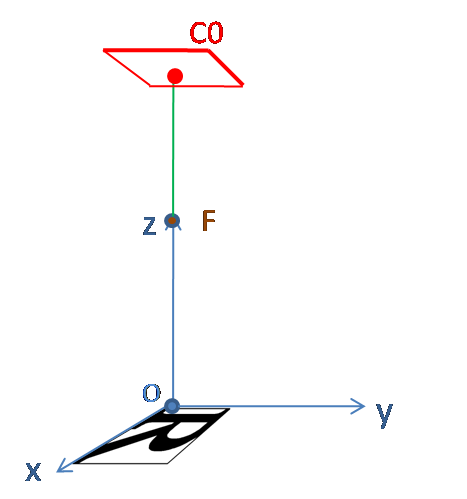
\includegraphics[scale=0.5]{vue_tps_identity.png}}}\\
		\subfigure[Vue après une première rotation (d'angle $\phi$)]{
		{
\includegraphics[width=60mm]{vue_fps_rotation_phi.jpg}}
		{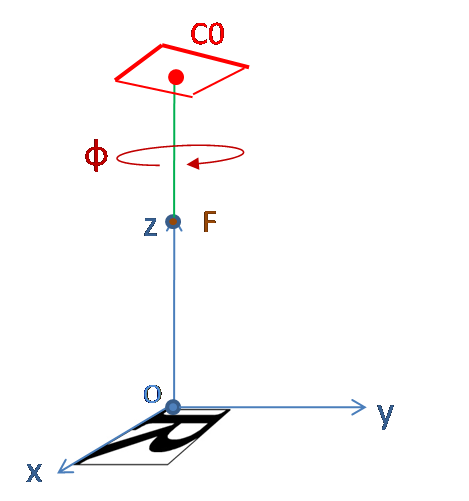
\includegraphics[scale=0.5]{vue_tps_rotation_phi.png}}}\\
		\subfigure[Vue après l'homographie particulière]{
		{
\includegraphics[width=60mm]{vue_fps_hom_part.jpg}}
		{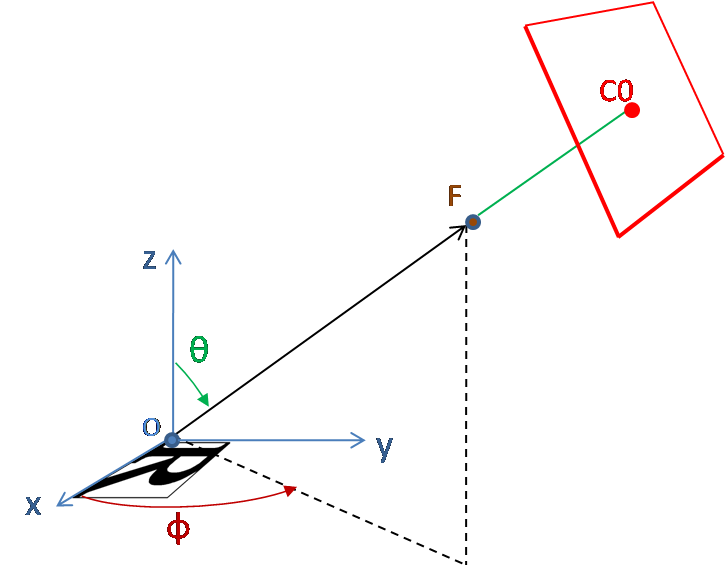
\includegraphics[scale=0.5]{vue_tps_hom_part.png}}}\\
		\subfigure[Vue finale (après rotation d'angle $\psi$)]{
		{
\includegraphics[width=60mm]{vue_fps_rotation_psi.jpg}}
		{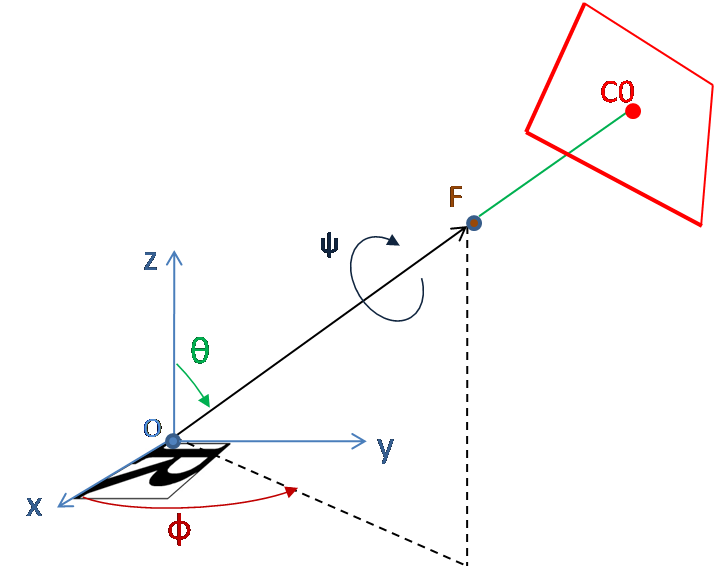
\includegraphics[scale=0.5]{vue_tps_rotation_psi.png}}}
		\caption{Étapes de traitement d'une homographie, assimilées à des mouvements de caméra (à gauche la vue de la caméra, à droite une vue extérieure immobile). Sur les vues extérieures, $F$ représente le point focal de la caméra, le plan rouge est le plan image de la caméra}
	\end{figure}
\clearpage
%simon
		\subsection{Traitement des homographies unidirectionnelles}
			\label{HomoboxRipmap}
			% contient la description des différentes possibilités pour traiter l'homographie particulière au centre de la décomposition
%simon
\subsubsection{Séparation d'une homographie particulière }

On considère une homographie $h$ de la forme 
\begin{equation*}
h:(x,y)\mapsto \left(\frac{-bx}{1-ax},\frac{-y}{1-ax}\right)
\end{equation*}
On peut décomposer cette homographie en deux applications $h_1 , h_2$
\begin{equation*}
h_1:(x,y) \mapsto \left(\frac{-bx}{1-ax}    ,y\right)~~~~~~h_2:(x,y) \mapsto \left(x,\frac{-y}{1-ax}\right)
\end{equation*}
On obtient $h=h_1  \circ h_2$, ce qui nous donne le schéma suivant 
\begin{equation*}
f\longrightarrow f'=f\circ h_1 \longrightarrow f''=f'\circ h_2
\end{equation*}
Chacune de ces deux transformations ne modifie l'image que dans une seule direction, cela permet d'effectuer des opérations sur des signaux unidimentionnels . Cette méthode n'est en revanche pas séparable.\\ 
La première transformation est une homographie en une dimension que l'on doit réaliser sur chaque ligne.\\ %sur ?
La seconde est un zoom d'un facteur différent sur chaque colonne.

\paragraph{Différentes méthodes de ré-échantillonage naif :}
%peut etre inutile
Le but ici est de présenter plusieurs méthodes permettant réaliser l'homographie par séparation.

\subparagraph{Méthode du point le plus proche :}
Il s'agit de la méthode la plus basique pour effectuer un ré-échantillonnage. On interpole l'image  par une fonction constante par morceau et on réévalue l'image $F\circ h $. Cette méthode est séparable, c'est-à-dire qu'il revient d'effectuer l'homographie $h$ et les deux applications $h_1 , h_2$ successivement.

\subparagraph{Méthode d'interpolation bilinéaire}
Cette méthode permet de réduire l'\emph{aliasing} par rapport à la méthode du point le plus proche, on interpole l'image en utilisant une fonction affine par morceaux $F$ et on évalue ensuite $F\circ h$. Cette méthode est aussi séparable.

%a étoffer
\paragraph{Sous échantillonnage gaussien :}
Dans le cas d'un zoom gaussien on utilise la convolution $f*G_{d}$. Le paramètre $d$ doit être choisi tel que 
\begin{equation*}
z^2 c^2=c^2 + d^2     ~~~~~~~c= 0.8
\end{equation*}
On obtient donc la formule $d=c\sqrt{z^2 - 1}$, nous renvoyons à l'article \cite{morel2011sift} pour les détails de ce raisonnement et une justification de la valeur expérimentale de c.\\

\paragraph{Sous échantillonnage utilisant les images intégrale }
Soit $d>0$, on veut convoler une fonction d'une variable par une approximation d'une gaussienne d'écart type $\delta$.\\
Soit $g_n^d$ le noyau défini par 
\begin{equation*}
g_1^d(t)=\frac{1}{d}\mathds{1}_{]-\frac{d}{2},\frac{d}{2}[}(t) ~~~~~~~g_{n+1}^d= g_n^d * g_1^d
\end{equation*}
Si on pose $G_n^d(x)=\sqrt{n}g_n^d(\sqrt{n} x)$ on peut montrer que 
\begin{equation*}
\widehat{G_n^d}(\omega)\underset{n\rightarrow\infty}{\rightarrow} \exp\left(-\frac{\omega^2 d^2}{12}\right)
\end{equation*}
\begin{proof}
On a $\widehat{g_1^d}(\omega)=\text{sinc}\left(\frac{\omega d}{2}\right)~~$  donc $~~\widehat{g_n^d}(\omega)=\text{sinc}\left(\frac{\omega d}{2}\right)^n~~$ et 
$~~\widehat{G_n^d}(\omega)=\text{sinc}\left(\frac{\omega d}{2\sqrt{n}}\right)^n~~$\\
on obtient le résultat voulu en réalisant un développement limité de cette fonction 
\end{proof}
Si $f,g$ sont deux fonctions continues à support compact et $d>0$ on a le résultat suivant
\begin{equation*}
(f*(g*g_1^d))(y)=\frac{(F^{(1)}*g)(y+\frac{d}{2})-(F^{(1)}*g)(y-\frac{d}{2})}{d}~~~~~~F^{(1)}(x)=\int_{-\infty}^{x}f(y) dy
\end{equation*}
\begin{proof}
Par intégration par partie (au sens des distributions), comme les fonctions $f$ et $g$ sont à support compact on obtient  :
\begin{eqnarray*}
(f * g *g_1^d )(y)&=&\frac{1}{d} \int_{\mathbb{R}} f(x)~(g * \mathds{1}_{]-\frac{d}{2},\frac{d}{2}[})(y-x) dx\\
                 &=& -\frac{1}{d} \int_{\mathbb{R}} F^{(1)}(x)~(g * (-\delta_{\frac{d}{2}}+\delta_{-\frac{d}{2}}))(x-y) dx\\
                 &=& \frac{1}{d} \int_{\mathbb{R}} F^{(1)}(x)~g(x-y-\frac{d}{2} )dx -\frac{1}{d} \int_{\mathbb{R}} F^{(1)}(x)~g(x-y+\frac{d}{2})dx\\
                 &=& \frac{(F^{(1)} * g)(y+\frac{d}{2})-(F^{(1)} * g )(y-\frac{d}{2})}{d}
\end{eqnarray*}
\end{proof}
On peut poser $D_d$ l'opérateur de "dérivation discrète" définit par $D_d f=f*\frac{f(.+\frac{d}{2})-f(.-\frac{d}{2})}{d}$ et réécrire la formule précédente 
\begin{equation*}
f * g *g_1^d =D_d (F^{(1)}*g)
\end{equation*}
On en déduit par récurrence la formule 
\begin{equation*}
(f*g_n^d)(y)=D_d ^n F^{(n)}= \frac{1}{d^n}\underset{0 \le k\le n}{\sum} \binom{n}{k}(-1)^{k} F^{(n)}(y+\frac{(n-2k)d}{2})
\end{equation*}
La fonction $F^{(k)}$ est la somme de la fonction  $F^{(k-1)}$, la seconde égalité se démontre en développant l'opérateur $D_d ^n$ par la formule du binome de Newton.\\
Dans nos algorithmes  on utilisera cette formule pour $n=3$ :
\begin{equation*}
(f*g_3)(y)=\frac{1}{d^3}(F^{(3)}(y+\frac{3d}{2})-3F^{(3)}(y+\frac{d}{2})+3F^{(3)}(y-\frac{d}{2})-F^{(3)}(y-\frac{3d}{2}))
\end{equation*}
On doit cependant calculer une valeur approchée des fonctions $F^{(k)}$  car on ne connait que les échantillons de la fonctions $f$.\\
On peut utiliser la méthode suivante on pose par récurrence
\begin{equation*}
F^{(n+1)}(k)=\underset{l\le k-1}{\sum}F^{(n)}(l)
\end{equation*}
On utilise ensuite une méthode d'interpolation par splines cubiques afin de pouvoir évaluer cette fonction en des valeurs non entière.\\
Une autre méthode consiste à poser 

\begin{equation*}
F^{(0)} (x) =\underset{0\le k \le m-1}{\sum}f_{k} \mathds{1}_{[k,k+1[}(x)
\end{equation*}
$(f_k)_{k=0...m-1}$ sont les termes du signal .On calcule ensuite $F^{(n)}(x)=\int_{-\infty}^{x}F^{(n-1)}(y)dx$ on à par exemple
\begin{equation*}
F^{(1)}(x)=\underset{k\le \lfloor x\rfloor \wedge m~-1}{\sum}f_{k}~~+ f_{\lfloor x\rfloor}
(x-\lfloor x\rfloor)
\end{equation*}
Cette fonction est affine par morceau on peut démontrer la formule suivante par récurrence \begin{equation*}
F^{(n)}(x)=F^{(n)}(\lfloor x\rfloor \wedge m)~~+\mathds{1}_{[0,m[}(x) \underset{0\le k \le n-1}{\sum}F^{(k)}(\lfloor x \rfloor) \frac{(x-\lfloor x \rfloor)^{n-k}}{(n-k)!}~~+\mathds{1}_{[m,+\infty[}(x)\underset{1\le k \le n-1}{\sum}F^{(k)}(m) \frac{(x-m)^{n-1-k}}{(n-1-k)!}
\end{equation*}
Où la valeur de $F^{(n)}$ se calcule par récurrence on a la relation $\forall k\le m$
\begin{equation*}
F^{(n)}(k+1)=F^{(n)}(k)+\underset{0\le l < n}{\sum} \frac{F^{(l)}(k)}{(n-l)!}
\end{equation*}
Comme dans la méthode précédente on doit calculer une composante constante par morceaux afin d'avoir la valeur de $F^{(n)}$ aux entiers  ainsi qu'un terme polynomial de degré $n$ pour effectuer l'interpolation sur des valeurs non-entières.\\
Dans le cas $n=3$ on obtient les formules
\begin{eqnarray*}
F^{(3)}(x)&=&F^{(3)}(\lfloor x\rfloor \wedge m)~~+\mathds{1}_{[0,m[}(x)(x-\lfloor x \rfloor) \left(F^{(2)}(\lfloor x \rfloor)+ \frac{(x-\lfloor x \rfloor)}{2}\left(F^{(1)}(\lfloor x \rfloor)+\frac{(x-\lfloor x \rfloor)}{3} f_{\lfloor x \rfloor}\right)\right)\\
          &+&\mathds{1}_{[m,+\infty[}(x)(x-\lfloor x \rfloor) \left(F^{(2)}(m)+ \frac{(x-\lfloor x \rfloor)}{2}F^{(1)}(m)\right) \\
F^{(3)}(k)&=&  \underset{0\le l<k}{\sum}\left(F^{(2)}(l)+\frac{F^{(1)}(l)}{2}+\frac{f_{l}}{6} \right)  \\
F^{(2)}(k)&=&  \underset{0\le l<k}{\sum}\left(F^{(1)}(l)+\frac{f_{l}}{2} \right)  \\
F^{(1)}(k)&=&  \underset{0\le l<k}{\sum}f_{l} 
\end{eqnarray*}
Si on fixe $0\le l\le m-1$ et on pose
\begin{equation*}
P_l (x)=F^{3}(l) +(x-l) \left(F^{(2)}(l)+ \frac{(x-l)}{2}\left(F^{(1)}(l)+\frac{(x-l)}{3} f_{l}\right)\right)
\end{equation*}
On obtient alors
\begin{eqnarray*}
P_l (l) &=& F^{(3)}(l) \\
P_l (l+1) &=& F^{(3)}(l+1) \\
P_l '(l) &=& F^{(2)}(l) \\
P_l '(l+1) &=& F^{(2)}(l+1)
\end{eqnarray*}
On peut donc obtenir ces formules en utilisant une méthode d'interpolation de Hermite. La fonction $F^{(3)}$ est la spline de cubique passant par le point $F^{(3)}(k)$ en $k$ avec une dérivé égale à $F^{(2)}(k)$, elle est $\mathcal{C}^2$.\\
Cette méthode a cependant un défaut, l'image est initialement interpolé par une fonction constante par morceau, on a donc utiliser une interpolation linéaire du signal de départ 
\begin{equation*}
F_1 ^{(0)}(x)=\underset{0\le k \le m-1}{\sum} f_k g_2^1 (x-k-\frac{1}{2})=(F_0^{(0)} *g_1^1 )(x)
\end{equation*}
On obtient alors 
\begin{equation*}
F_1 ^{(0)}*g_n^d=(F_0 ^{(0)}*g_1^1)*g_n^d=(F_0 ^{(0)}*g_n^d)*g_1^1=(D_d^n F_0 ^{(n)})*g_1^1=D_1 D_d^n F_0^{(n+1)}
\end{equation*}
L'interpolation supplémentaire peut donc être obtenue en évaluant $F_0^{(n+1)}$. La méthode de calcul est donc la même que dans le cas précédent.\\
Il est possible d'utiliser cette méthode pour obtenir une représentation $F_n^{(0)}$ plus régulière du signal de départ mais la courbe n'est pas  interpolante si $2\le n$.\\
%à faire mieux 
Afin d'implémenter cette méthode nous devons déterminer la valeur du paramètre $d$ en fonction du facteur de zoom local. Nous allons réutiliser les résultats du paragraphe précédent, car la fonction $g_3$ est une bonne approximation d'une gaussienne. L'écart type de $g_1$ est $\sigma_1=\frac{d}{\sqrt{12}}$ donc l'écart type $\sigma_3$ est donné par la formule $\sigma_3=\sqrt{3}\sigma_1=\frac{d}{2}$
donc $d=2c\sqrt{z^2 - 1}$.\\
Dans la pratique on utilisera la formule $d=2\sqrt{(0.8)^2 z^2 - (0.7)^2}$ car les images utilisées ne sont en général pas parfaites.\\

\paragraph{Sur-échantillonage par splines :}
%Pas encore fait
\subparagraph{Splines cubiques de Hermite :}
Si $(x_0,x_1,x_2,x_3)$ et $(y_0,y_1,y_2,y_3)$  permet de construire un polynôme $P$ de degrès 3 tel que  
\begin{equation*}
P(x_1)=y_1~~~~P(x_2)=y_2~~~~P'(x_1)= \frac{y_2-y_0}{x_2 -x_0}~~~~P'(x_2)= \frac{y_3-y_1}{x_3 -x_1}
\end{equation*}
%simon
		\subsection{Traitement des rotations}
			\label{YaroSzeli}
			% contient la description des différentes méthodes pour traiter les rotations de la décomposition

Pour les deux rotations dans la décomposition, nous avons testés plusieures méthodes : la méthodes de Yaroslavsky \cite{unser1995convolution} et la méthode de traitement des affinités multiétapes \cite{szeliski2010high}.

\subsubsection{Méthode de Yaroslavsky}

La méthode de Yaroslavsky consiste à décomposer une rotation en trois "shear".//

Sous forme matricielle un rotation s'écrit de manière générale :
\begin{equation*}
	H=\begin{pmatrix}
	cos \theta&-sin \theta\\sin \theta&cos \theta
	\end{pmatrix}
	\end{equation*}

La décomposition en trois shear est la suivante :
\begin{equation*}
	H=\begin{pmatrix}
	cos \theta&-sin \theta\\sin \theta&cos \theta
	\end{pmatrix}=\begin{pmatrix}
	1&-tan \frac{\theta}{2}\\0&1
	\end{pmatrix}\begin{pmatrix}
	1&0\\sin \theta&1
	\end{pmatrix}\begin{pmatrix}
	1&-tan \frac{\theta}{2}\\0&1
	\end{pmatrix}
	\end{equation*}

	Pour faire la rotation complète on fait chaque shear par fourier et on recentre l'image après chaque shear.\\
	En pratique on se ramène toujours à des rotations d'angle entre $[\frac{-\pi}{4},\frac{\pi}{4}]$ (on peut en effet faire des rotations d'angle $\pi$ et $\frac{\pi}{2}$ de manière exacte...)  
 %Jean-Thomas à fait une partie sur Yaroslavsky...
	\clearpage
	\section*{Conclusion}
			%ici une conclusion chouette

La décomposition géométrique permet ainsi une réalisation des homographies de meilleure qualité, et un contrôle plus rigoureux de l'\emph{aliasing} et du flou introduit. Les solutions proposées ici pour implémenter les différentes étapes ne sont que des exemples. Elles sont coûteuses en calcul bien que linéaires. 

On peut ainsi imaginer des approximations moins satisfaisantes mais beaucoup plus rapide, par exemple en utilisant une méthode triple intégrale pour les rotations. De même le traitements de l'homographie unidirectionnelle peut-être simplifié, par exemple en n'intégrant que sur les entiers et en réalisant une interpolation bilinéaire.

On a ainsi proposé une décomposition géométrique des homographies autour de laquelle de nombreux algorithmes peuvent s'articuler.

%probablement un peu trop emphatique, n'hésitez pas à y retoucher ! 

	\clearpage
	\section{Expériences}
		\label{experiences}
		% contient les différentes comparaisons entre les différentes méthodes

% éléments à comparer :
%   - méthode naïve
%   - MipMap
%   - RipMap (différentes distances ?)
%   - geo_qqlch_homobox
%   - geo_qqlch_ripmap
%   - geo_szeli_truc
%   - geo_yaro_truc
% avec "qqlch" = "szeli" ou "yaro" (à choisir) et "truc" = "homobox" ou "ripmap" (à choisir)

		%pour l'instant on ajoute nos experiments chacun en vrac, on verra l'ordre quand on aura tout
		\subsection{Décomposition multi-étapes d'une affinité}
 
 On présente ici les résultats de la décomposition multi-étapes d'une affinité \cite{szeliski2010high} (section \ref{szeliski_section}), ainsi que le spectre de l'image aux différentes étapes. L'affinité utilisée étant elle même un \emph{shear}, la décomposition en six étapes élémentaires se réduit à trois étapes élémentaires. La réduction à quatre étapes n'a donc pas lieu d'être, on reste donc à trois étapes élémentaires.
 
	\begin{figure}
		\centering
		\subfigure[Image initiale (échelle 3/8)]{
			{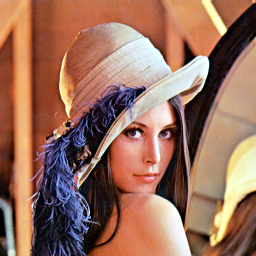
\includegraphics[scale=0.375]{decompoSzeliski_sinc_image_entree.png}}
			{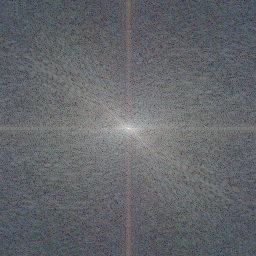
\includegraphics[scale=0.375]{decompoSzeliski_sinc_fourier_entree.png}}
		}
		\subfigure[Image plongée dans une image neuf fois plus grande (échelle 1/8)]{
			{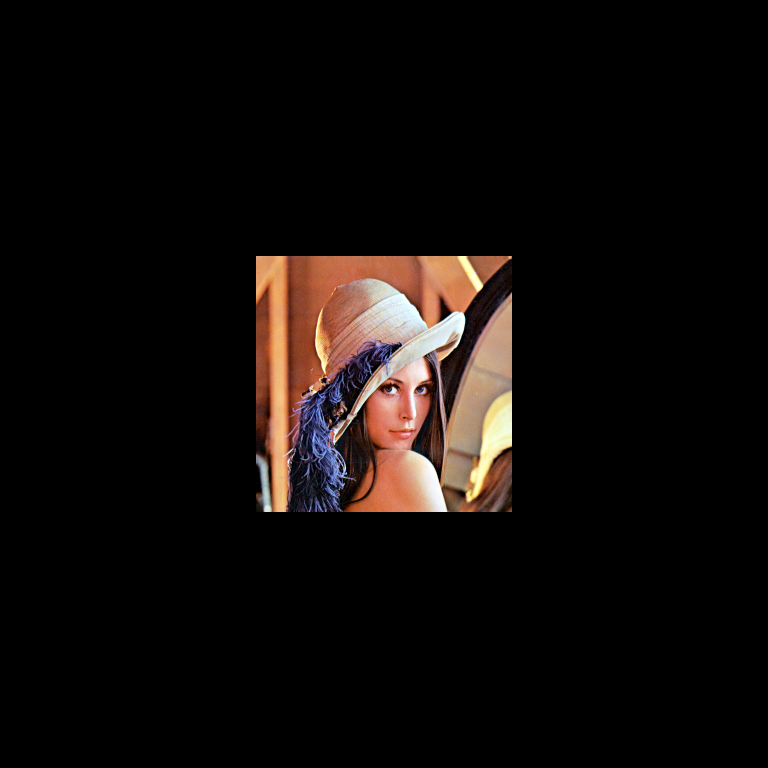
\includegraphics[scale=0.125]{decompoSzeliski_sinc_image1.png}}
			{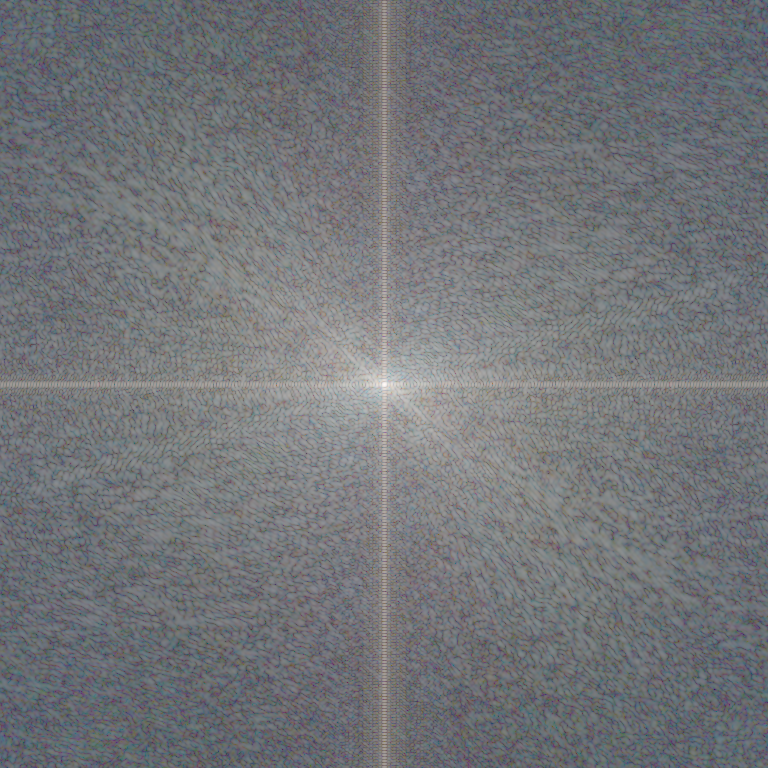
\includegraphics[scale=0.125]{decompoSzeliski_sinc_fourier1.png}}
		}
		\subfigure[Après le premier $\mathcal R$ (échelle 1/8)]{
			{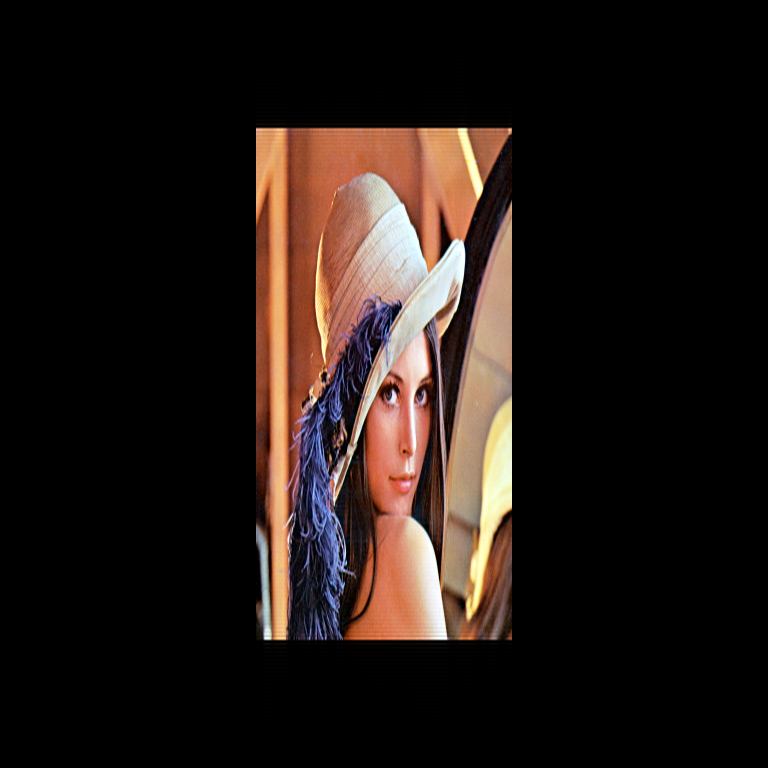
\includegraphics[scale=0.125]{decompoSzeliski_sinc_image2.png}}
			{
\includegraphics[scale=0.125]{decompoSzeliski_sinc_fourier2.png}}
		}
		\subfigure[Après le deuxième $\mathcal R$ (échelle 1/8)]{
			{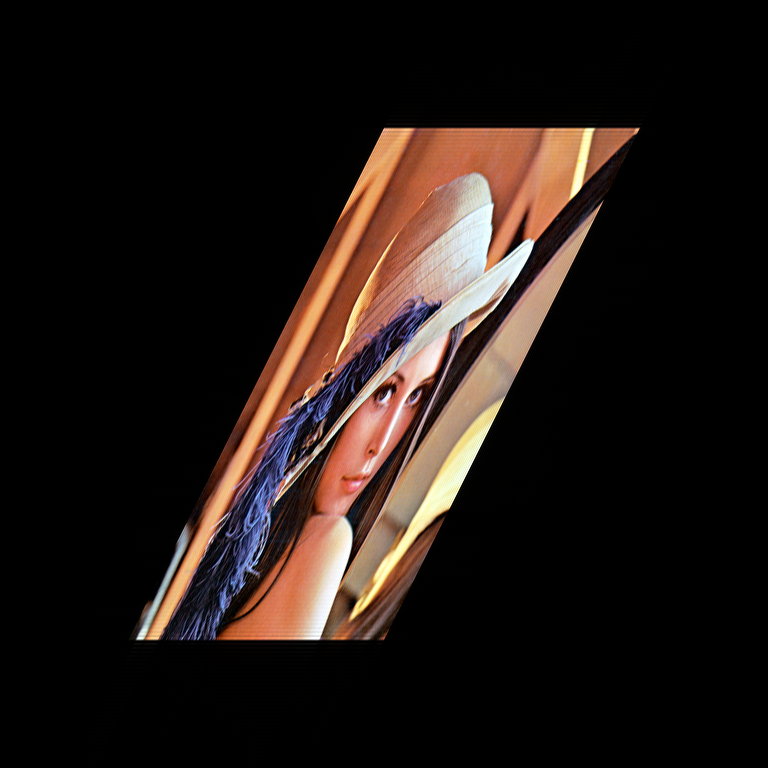
\includegraphics[scale=0.125]{decompoSzeliski_sinc_image3.png}}
			{
\includegraphics[scale=0.125]{decompoSzeliski_sinc_fourier3.png}}
		}
		\subfigure[Après le troisième $\mathcal R$ (échelle 1/8)]{
			{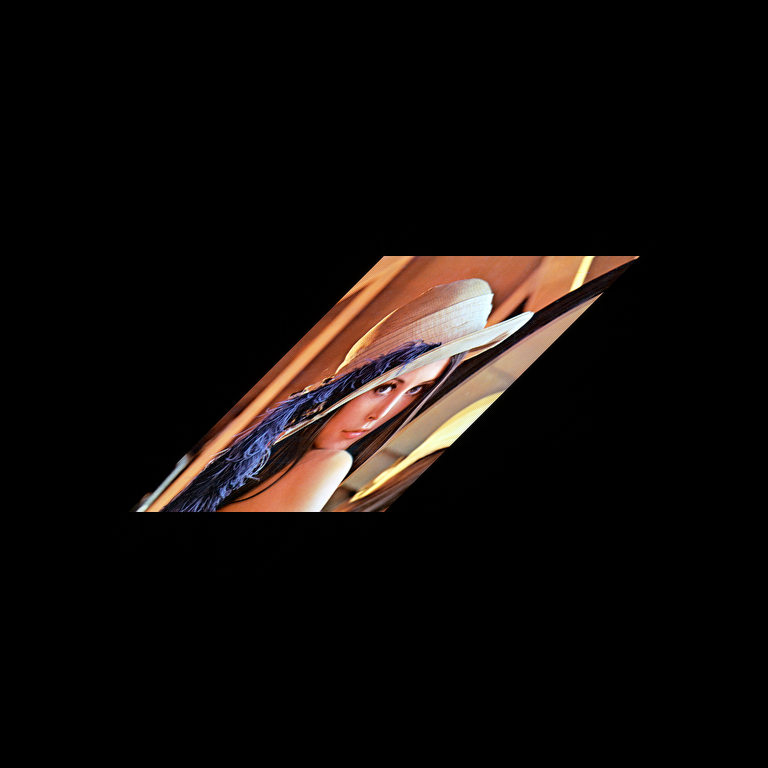
\includegraphics[scale=0.125]{decompoSzeliski_sinc_image4.png}}
			{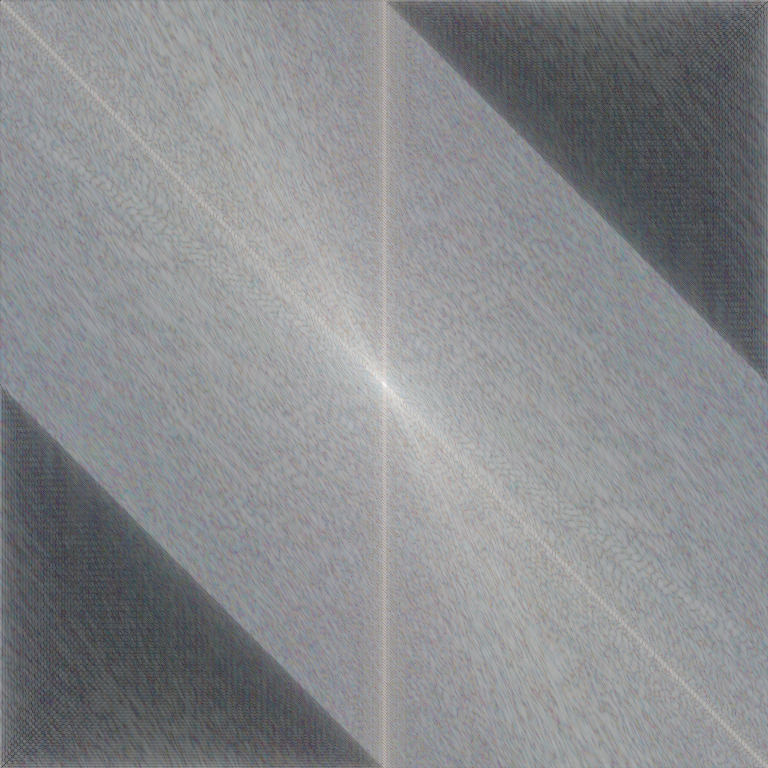
\includegraphics[scale=0.125]{decompoSzeliski_sinc_fourier4.png}}
		}
		\subfigure[Image finale (échelle 3/8)]{
			{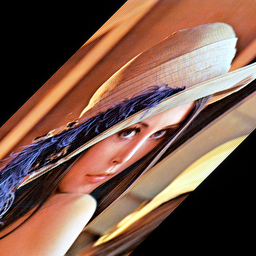
\includegraphics[scale=0.375]{decompoSzeliski_sinc_image_sortie.png}}
			{
\includegraphics[scale=0.375]{decompoSzeliski_sinc_fourier_sortie.png}}
		}
		\caption{Étapes du traitement des affinités présenté en \ref{szeliski_section} (à gauche l'image à chaque étape, à droite le logarithme du module de la transformée de Fourier de cette image). Le filtre d'interpolation est un \emph{sinc} (de période 1)}
		\label{experiments_decompoSzeliski_sinc}
	\end{figure}
	
	En figure \ref{experiments_decompoSzeliski_sinc}, le filtre utilisé est un \emph{sinc}, correspondant au \emph{raised cosine-weighted sinc} avec $\beta = 0$ ; pour rappel, le filtre a pour forme
	\[h : x \mapsto \sinc(\frac{x}{T})\frac{\cos(\frac{\pi\beta x}{T})}{1-\frac{4\beta^2x^2}{T^2}}\]
	On ne perd pas en qualité visuelle en réduisant la convolution à un nombre fini de termes suffisamment grand, par exemple 90.
	
	Avec un $\beta$ plus élevé, on conserve des hautes fréquences sur l'extérieur du spectre, mais dont l'impact est faible quand l'image reprend sa taille initiale ; en augmentant $\beta$ (figure \ref{experiments_decompoSzeliski}), on peut donc autoriser un peu plus de repliement du spectre, en veillant à ce que visuellement, on n'observe aucun artefact. Comme l'augmentation de $\beta$ augmente la vitesse à laquelle le filtre décroit, on peut alors convoler sur des supports plus réduits, et donc gagner du temps. Avec $\beta = 0.36$, on peut restreindre la convolution à une somme de 9 termes (figure \ref{szeliski_plotRaisedCosine}) (9 est le nombre de termes de base ; il est plus grand lors des sur-échantillonnages car le support du filtre de convolution est adaptatif). Cette valeur $\beta = 0.36$ est celle qu'on utilise pour les autres expériences.
 
	\begin{figure}
		\centering
		\subfigure[Image initiale (échelle 3/8)]{
			{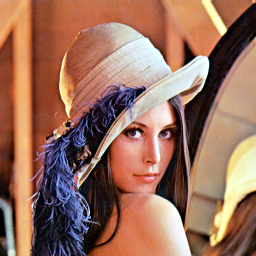
\includegraphics[scale=0.375]{decompoSzeliski_image_entree.png}}
			{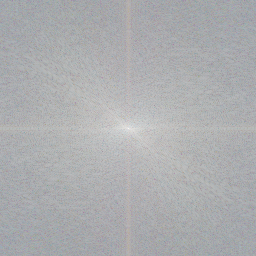
\includegraphics[scale=0.375]{decompoSzeliski_fourier_entree.png}}
		}
		\subfigure[Image plongée dans une image neuf fois plus grande (échelle 1/8)]{
			{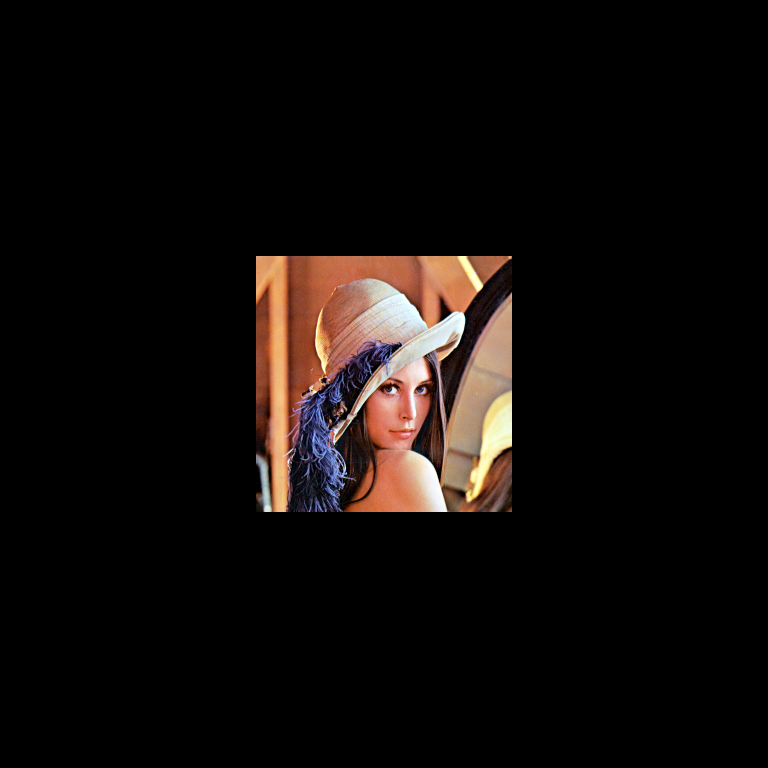
\includegraphics[scale=0.125]{decompoSzeliski_image1.png}}
			{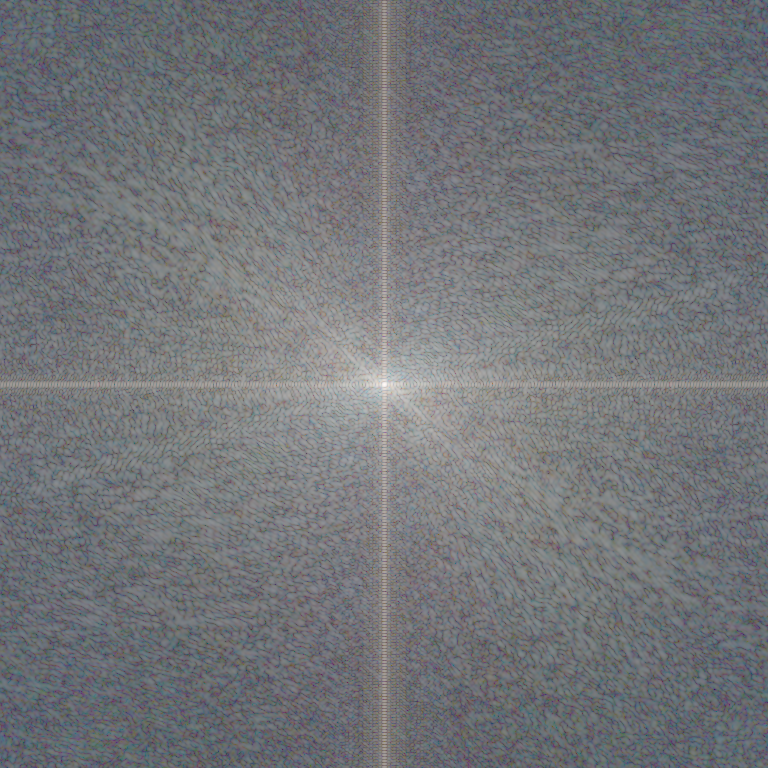
\includegraphics[scale=0.125]{decompoSzeliski_fourier1.png}}
		}
		\subfigure[Après le premier $\mathcal R$ (échelle 1/8)]{
			{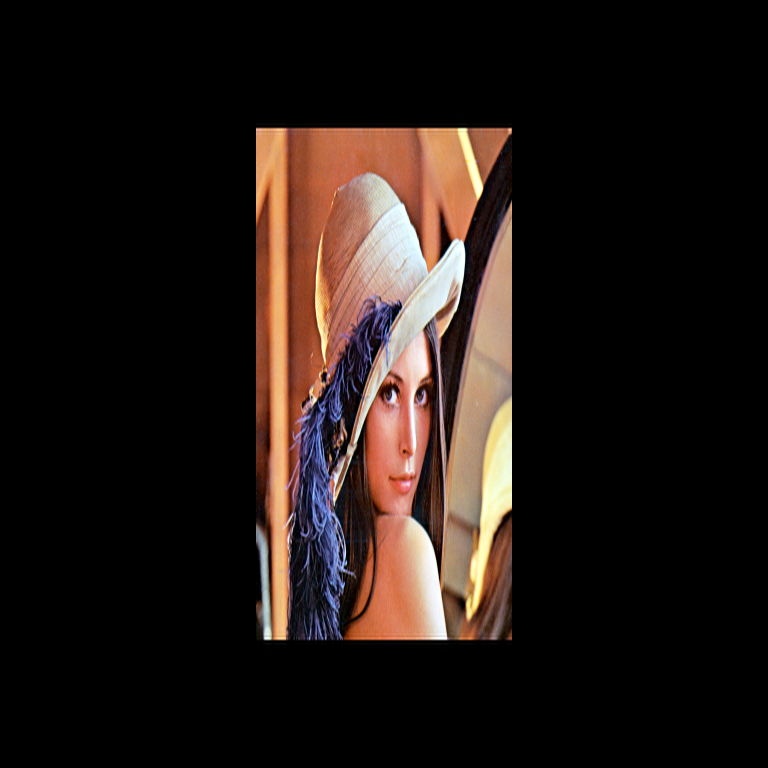
\includegraphics[scale=0.125]{decompoSzeliski_image2.png}}
			{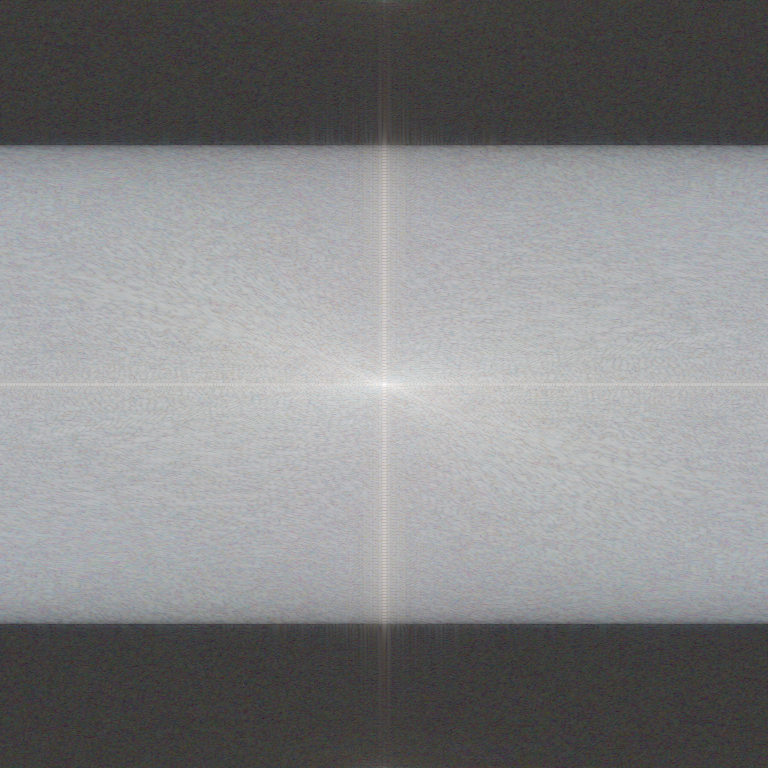
\includegraphics[scale=0.125]{decompoSzeliski_fourier2.png}}
		}
		\subfigure[Après le deuxième $\mathcal R$ (échelle 1/8)]{
			{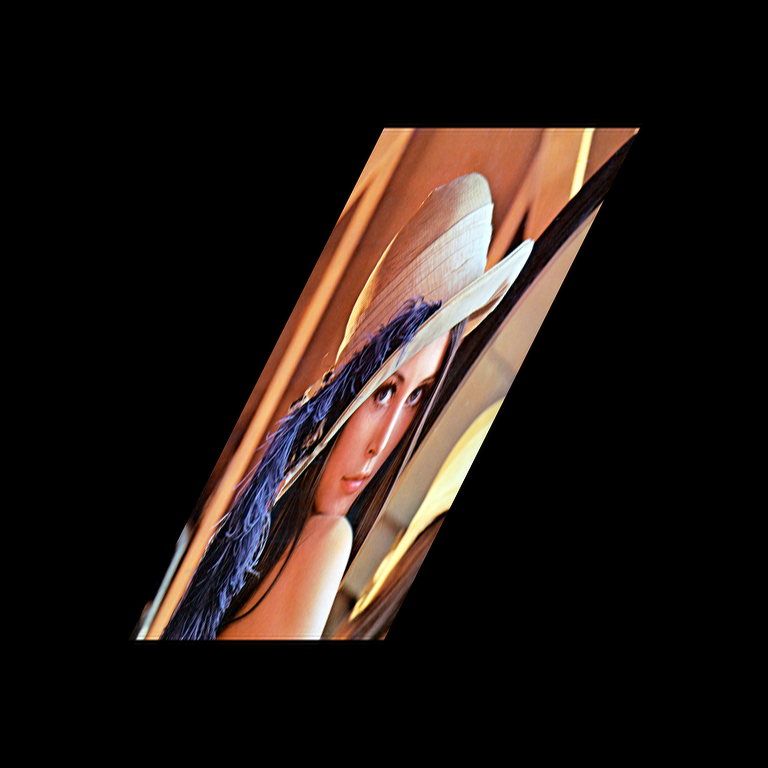
\includegraphics[scale=0.125]{decompoSzeliski_image3.png}}
			{
\includegraphics[scale=0.125]{decompoSzeliski_fourier3.png}}
		}
		\subfigure[Après le troisième $\mathcal R$ (échelle 1/8)]{
			{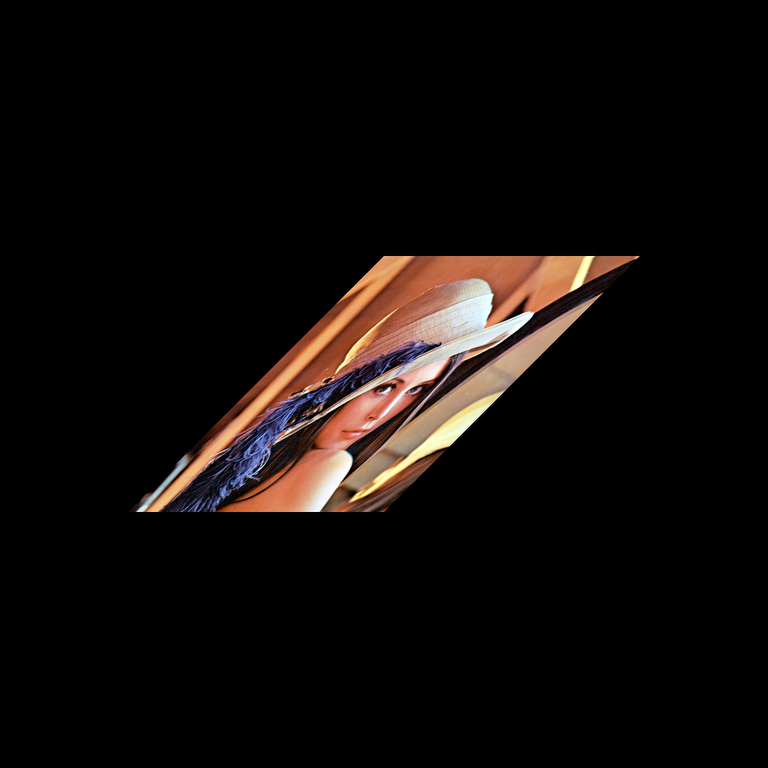
\includegraphics[scale=0.125]{decompoSzeliski_image4.png}}
			{\includegraphics[scale=0.125]{decompoSzeliski_fourier4.png}}
		}
		\subfigure[Image finale (échelle 3/8)]{
			{\includegraphics[scale=0.375]{decompoSzeliski_image_sortie.png}}
			{\includegraphics[scale=0.375]{decompoSzeliski_fourier_sortie.png}}
		}
		\caption{Étapes du traitement des affinités présenté en \ref{szeliski_section} (à gauche l'image à chaque étape, à droite le logarithme du module de la transformée de Fourier de cette image). Le filtre d'interpolation est un \emph{raised cosine-weighted sinc} (de période 1, de \emph{roll-off factor} $\beta = 0.25$)}
		\label{experiments_decompoSzeliski}
	\end{figure}

		%contient des exemples d'homographies traité par nous et ripmap

\sse{Comparaison du Ripmap et de la décomposition géométrique}

Se reporter aux figures \ref{Homo1},\ref{Homo2},\ref{Homo3} et \ref{Homo4}.

On peut remarquer que la décomposition permet pour certaines homographies de limiter l'\emph{aliasing} (Homographies 1 et 4). Dans le cas d'une déformation en diagonale elle limite le flou (Homographie 2). Il existe néanmoins des cas où les deux méthodes ont des performances comparables (Homographie 3).

\begin{figure}
\subfigure[Décomposition géométrique]{\includegraphics[scale=0.4]{img_f_1.png}}
\subfigure[Ripmap]{\includegraphics[scale=0.4]{img_ripmap_1.png}}
\caption{Homographie 1 : La décomposition géométrique produit moins d'\emph{aliasing}}
\label{Homo1}
\end{figure}

\begin{figure}
\subfigure[Décomposition géométrique]{\includegraphics[scale=0.4]{img_f_2.png}}
\subfigure[Ripmap]{\includegraphics[scale=0.4]{img_ripmap_2.png}}
\caption{Homographie 2 : La décomposition n'entraine pas d'\emph{over-blurring} (voir section \ref{Ripmap})}
\label{Homo2}
\end{figure}

\begin{figure}
\subfigure[Décomposition géométrique]{\includegraphics[scale=0.4]{img_f_3.png}}
\subfigure[Ripmap]{\includegraphics[scale=0.4]{img_ripmap_3.png}}
\caption{Homographie 3 : Aucune des deux méthodes n'est clairement meilleure}
\label{Homo3}
\end{figure}

\begin{figure}
\subfigure[Décomposition géométrique]{\includegraphics[scale=0.4]{img_f_4.png}}
\subfigure[Ripmap]{\includegraphics[scale=0.4]{img_ripmap_4.png}}
\caption{Homographie 4 : La décomposition géométrique produit moins d'\emph{aliasing}}
\label{Homo4}
\end{figure}

\begin{figure}
\subfigure[Décomposition géométrique]{\includegraphics[scale=0.4]{img_geo_5.png}}
\subfigure[Ripmap]{\includegraphics[scale=0.4]{img_ripmap_5.png}}
\subfigure[Méthode naive]{\includegraphics[scale=0.4]{img_naive_5.png}}
\subfigure[Mipmap]{\includegraphics[scale=0.4]{img_mipmap_5.png}}
\caption{Homographie 5 : La décomposition produit moins d'aliasing, un détail est présenté dans la figure \ref{Homo5det}}
\label{Homo5}
\end{figure}

\begin{figure}[t]
\centering
\subfigure[Méthode naive]{\includegraphics[scale=1.25]{img_det_naive.png}}\hfill
\subfigure[Mipmap]{\includegraphics[scale=1.25]{img_det_mipmap.png}}\hfill
\subfigure[Ripmap]{\includegraphics[scale=1.25]{img_det_ripmap.png}}\hfill
\subfigure[Décomposition géométrique]{\includegraphics[scale=1.25]{img_det_geo.png}}
\caption{Détail de l'homographie 5 qui a été présentée dans la figure \ref{Homo5}}
\label{Homo5det}
\end{figure}
	\clearpage
	\appendix
	\label{pseudo_code}
	\section{Pseudo-code pour le Mipmap et le Ripmap}
		%pseudo-code mipmap/ripmap
%Hugo s'en charge
\sse{Pseudo-code pour le Mipmap}

\ssse{Conventions}

Un Mipmap est un tableau à trois dimensions, avec les deux axes usuels et une profondeur $d$.
Ainsi $M[3]$ est le carré $4$ fois moins haut que l'image d'origine. On note $n=2^l$ la taille de l'image (qui est supposée carrée). On note $D$ la fonction de distance (à deux arguments).

On utilise la convention suivante pour la profondeur : 
\begin{itemize}
\item Si $d = 1$ alors on considère l'image d'origine.
\item Si $d = n$ alors on considère l'image d'un pixel qui est la moyenne de l'image.
\end{itemize}
%ici mettre une image symbolique, schéma de la pyramide avec u,v et d

En pratique, on a périodisé l'image.

\ssse{Pseudo-code}

Ici on a juste le corps de la fonction, ainsi la fonction de distance et la construction du mipmap ne sont pas précisées, ils le sont dans les sections suivantes.
\medbreak
\medbreak
\begin{algorithm}[H]
\caption{$mainFunction(img,H,img_f)$}
\KwData{Une image $img[1..n][1..n]$, Une homographie $H = \left( \begin{array}{ccc} a &b & p\\ c & d & q \\ r & s & t\\ \end{array}\right)$, une fenêtre d'arrivée $img_f[1..m][1..m]$}
$M=builtMipMap(img)$ \;%Faire le mip-mapping de $img$ noté $M$\;
Calculer l'homographie inverse $H^{-1}$ (et calculer la fonction $D$ de $x,y$ en même temps)\;
\For{$(x,y) \in \llb 1,m \rrb^2$}{
Calculer $d=D(x,y)$ \;%préciser les équations
$I[x][y] = evalPixel(H^{-1}(x,y),d,M)$\;
}
\KwRet{I}
\end{algorithm}

\medbreak
\medbreak
L'interpolation trilinéaire :
\medbreak
\medbreak

\begin{algorithm}[H]
\caption{$evalPixel((u,v),d,M)$}
\KwData{Des coordonnées $(u,v) \in \mb{R}^2$, une distance $d \in \mb{R}$, un mipmap $M[1..l]$ où chaque élément est un image}
\uIf{$d\leq1$}{\KwRet{$bilinearMipMap(u,v,M[1])$}}
\uElseIf{$d>l$}{\KwRet{$M[l][1][1]$}}
\Else{Trouver $m \in \mb{N}$ tels que $2^m \leq d < 2^{m+1}$\;
$a=bilinearMipMap(\frac{u}{2^{m-1}}, \frac{v}{2^{m-1}},M[m])$\;
$b= bilinearMipMap(\frac{u}{2^{m}}, \frac{v}{2^{m}},M[m+1])$\; 
\KwRet{$ (m+1 - \log (d)) a + (\log (d) - m) b$}}

\end{algorithm}

\medbreak
\medbreak
Ici l'interpolation bilinéaire, au niveau $d$.
\medbreak
\medbreak

\begin{algorithm}[H]
\caption{$bilinearMipMap((u,v),M)$}
\KwData{Des coordonnées $(u,v) \in \mb{R}^2$, une image tirée du mipmap $img[1..k][1..k]$}
$u'=floor(u)$\;
$v' = floor(v)$\;
$x=u-u'$\;
$y = v-v'$\;
\KwRet{$(1-x)(1-y)*img[u'][v'] + (1-x)y*img[u'][v'+1] + x(1-y)*I[u'+1][v']+xy*img[u'+1][v'+1]$}\;
\end{algorithm}

\medbreak
\medbreak
Ce n'est qu'un algorithme générique, nous allons maintenant voir comment le spécifier pour permettre une implémentation réelle. Il faut examiner la construction du mipmap. On s'est intéressé au problème de la fonction de distance dans la partie sur les méthodes existantes. %a voir mettre une reference / un lien...

\ssse{Construction du mipmap}

Voici un exemple naïf de construction d'un mipmap. On fait simplement la moyenne des quatre pixels concernés.
 \medbreak
  \medbreak
 \begin{algorithm}[H]
 \caption{$buildMipMap(img)$}
 \KwData{Une image $img[1..n][1..n]$ (où $n = 2^l$)}
 \For{$(i,j)\in \llb1,n\rrb^2$}{
 	$M[1][i][j]=img[i][j]$\;
 }
 \For{$u \in \llb 2,l+1\rrb$}{
 	\For{$(i,j)\in \llb1,\frac{n}{2^{u-1}}\rrb^2$}{
		$M[u][i][j]=\frac{M[u-1][2i][2j][u-1]+M[u-1][2i-1][2j]+M[u-1][2i][2j-1]+M[u-1][2i-1][2j-1]}{4}$\;
	}
 }
 \end{algorithm}
 \medbreak
  \medbreak
 Ce n'est pas une bonne méthode, en pratique on a fait précédé chaque moyennage par un filtrage gaussien de l'image. C'est une phase de précalcul, on tolère le fait qu'elle soit relativement coûteuse.  


\sse{Le ripmap}

\ssse{Conventions}

Le ripmap $R$ et quadri-dimensionnel  : les deux premiers indices indiquent le rectangle, les deux autres indiquent le pixel du rectangle. Ainsi appeler $R[2][4]$ appelle une image simple, de largeur $\frac{1}{2}$ et de hauteur $\frac{1}{16}$ de l'image d'origine. On suppose l'image de départ carrée de taille $n=2^l$.

\ssse{Pseudo-code pour le ripmap}

La fonction principale, très similaire au ripmap.
\medbreak
\medbreak
\begin{algorithm}[H]
\caption{$mainFunction(img,H,img_f)$}
\KwData{Une image $img[1..n][1..n]$, Une homographie $H = \left( \begin{array}{ccc} a &b & p\\ c & d & q \\ r & s & t\\ \end{array}\right)$, une fenêtre d'arrivée $img_f[1..m][1..m]$}
$R = buildRipMap(img)$\;
Calculer l'homographie inverse $H^{-1}$ (et précalculer les fonctions $\frac{\dr u}{\dr x},\frac{\dr u}{\dr y},\frac{\dr v}{\dr x},\frac{\dr v}{\dr y}$ de $x,y$ en même temps)\;
\For{$(x,y) \in \llb 1,m \rrb^2$}{
Calculer $d_1=|\frac{\dr u}{\dr x}(x,y)|+|\frac{\dr u}{\dr y}(x,y)|$ \;
Calculer $d_2=|\frac{\dr v}{\dr x}(x,y)|+|\frac{\dr v}{\dr y}(x,y)|$\;
Calculer $c_1 = \min(0,\frac{\dr u}{\dr x}(x,y))+\min(0,\frac{\dr u}{\dr y}(x,y))$\;
Calculer $c_2 = \min(0,\frac{\dr v}{\dr x}(x,y))+\min(0,\frac{\dr v}{\dr y}(x,y))$\;
$img_f[x][y] = evalPixel(H^{-1}(x,y)+(c_1,c_2),d_1,d_2,R)$\;
}
\KwRet{I}
\end{algorithm}

\medbreak
\medbreak

L'interpolation bilinéaire entre les rectangles.
Les $m_{ij}$ permettent de simplifier l'écriture des cas ou l'une des distances est trop grande ou trop petite :

\medbreak
\medbreak

\begin{algorithm}[H]
\caption{$evalPixel((u,v),d_1,d_2,M)$}
\KwData{Des coordonnées $(u,v) \in \mb{R}^2$, des distances $d_1,d_2 \in \mb{R}$, un Ripmap $R[1..l][1..l]$ constitué d'images}
\For{$i\in \llb 1,2\rrb$}{
$x_i = \floor{\log_2(d_i)}$\;
\uIf{$x_i \leq 1$}{$m_{i1}=m_{i2} = 1$\;}
\uElseIf{$x_i\geq l$}{$m_{i1}=m_{i2}=l$\;}
\Else{$m_{i1} = x_i -1$ \;$m_{i2} = x_i$\;}
}

$a=bilinearMipMap(\frac{u}{2^{m_{11}}},\frac{v}{2^{m_{21}}},R[m_{11}+1][m_{21}+1])$\;
$b=bilinearMipMap(\frac{u}{2^{m_{12}}},\frac{v}{2^{m_{21}}},R[m_{12}+1][m_{21}+1])$\;$c=bilinearMipMap(\frac{u}{2^{m_{11}}},\frac{v}{2^{m_{22}}},R[m_{12}+1][m_{22}+1])$\;
$d=bilinearMipMap(\frac{u}{2^{m_{12}}},\frac{v}{2^{m_{22}}},R[m_{12}+1][m_{22}+1])$\;

$x = m_{12} - \log_2(d_1)$\;
$y = m_{22} - \log_2(d_2)$\;

\KwRet{$xy * a + (1-x)y * b + x(1-y) * c + (1-x)(1-y) * d$\;}
\end{algorithm}


\ssse{La construction du ripmap}

On présente un algorithme naïf de construction de ripmap.
\medbreak
\medbreak
\begin{algorithm}[H]
\caption{buildRipMap(img)}
\KwData{une image $img[1..n][1..n]$, où $n = 2^l$}
$R[1][1] = img$\;
\For{$j\in\llb 2,l\rrb$}{
	\For{$(u,v)\in \llb 1,n\rrb \times \llb1,\frac{n}{2^{j-1}}\rrb$}{
		$R[1][j][u][v] = \frac{R[1][j-1][u][2v] + R[1][j-1][u][2v-1]}{2}$\;
	}
}

\For{$j\in\llb 1,l\rrb$}{
\For{$i\in\llb 2,l\rrb$}{
\For{$(u,v)\in \llb 1,\frac{n}{2^{i-1}}\rrb \times \llb1,\frac{n}{2^{j-1}}\rrb$}{
		$R[i-1][j][u][v] = \frac{R[i-1][j][2u][v] + R[i-1][j][2u-1][v]}{2}$\;
	}}}
\KwRet{$R$}
\end{algorithm}
\medbreak
\medbreak
Dans la pratique on a filtré à l'aide d'un filtre gaussien dans la direction où l'on compresse, et ce à chaque étape.
\medbreak
\medbreak
\begin{algorithm}[H]
\caption{buildRipMapGaussien(img)}
\KwData{une image $img[1..n][1..n]$, où $n = 2^l$}
$R[1][1] = img$\;
\For{$j\in\llb 2,l\rrb$}{
	\For{$(u,v)\in \llb 1,n\rrb \times \llb1,\frac{n}{2^{j-1}}\rrb$}{
		$R[1][j][u][v] = convolutionHorizontale(R[1][j-1])[u][2v]$\;
	}
}

\For{$j\in\llb 1,l\rrb$}{
\For{$i\in\llb 2,l\rrb$}{
\For{$(u,v)\in \llb 1,\frac{n}{2^{i-1}}\rrb \times \llb1,\frac{n}{2^{j-1}}\rrb$}{
		$R[i-1][j][u][v] = convolutionVerticale(R[i-1][j])[2u][v]$\;
	}}}
\KwRet{$R$}
\end{algorithm}
\medbreak
\medbreak
Où les fonctions $convolution$ convolent dans la direction indiquée par une gaussienne d'écart-type $1,4$ (se reporter à \cite{morel2011sift})


%hugo
	\section{Pseudo-code pour la décomposition géométrique}
		\subsection{Pseudo-code pour la décomposition d'une homographie}
 
 On rappelle que dans les algorithmes qui suivent, on prend la convention suivante : $H = \pmatrice{a&b&p\\c&d&q\\r&s&t}$ est la matrice carrée de taille 3 (ou l'application homographique) telle que si $img$ est l'image d'entrée et $img_f$ est l'image de sortie, $img_f(x) = img(H(x))$. Ainsi, la décomposition $H \sim T_{c} R_{\psi}  \tilde H R_{\phi}$ est exécutée de gauche à droite. On notera cette décomposition $A \tilde H B$, et ces trois matrices seront les objets renvoyés par $decomposition$.
 
 Cet algorithme $decomposition$ (algorithme \ref{pseudoCodeDecompo}) présente la décomposition correspondant aux schémas \ref{SchemaEtapesDecompoGeometrique}. Arbitrairement, on choisit le degré de liberté de sorte à annuler une des translations (verticale ou horizontale) de $T_c$ : pour cela, on rappelle que $(x_2,y_2)$ (nommés $t_0,t_1$ dans l'algorithme) doivent vérifier
 \[\Delta_H(x_2 , y_2 ) \stackrel{\text{déf}}{=} \hat r ((rc+sd)-(r^2 + s^2)y_2) - \hat s ((ar+sb)-(r^2 + s^2 )x_2) = 0 \]
 On prend donc $t_0 = x_2 = -\frac{\Delta_H(0,0)}{(r^2+s^2)\hat s}, t_1 = y_2 = 0$ ou $t_0 = x_2 = 0, t_1 = y_2 = -\frac{\Delta_H(0,0)}{(r^2+s^2)\hat r}$, en choisissant de sorte à ne pas diviser par zéro.
 
   \begin{algorithme}
     \label{pseudoCodeDecompo}
     \caption{$decomposition(H)$}
     \KwData{Une matrice d'homographie $H \in \mathcal M_{3,3}$}
     \eIf{$as-br\neq0$}{
      $t_0 = -\frac{\Delta_H(0,0)}{(r^2+s^2)\hat s}$\;
      $t_1 = 0$\;
     }{
      $t_0 = 0$\;
      $t_1 = -\frac{\Delta_H(0,0)}{(r^2+s^2)\hat r}$\;
     }
     $N_\phi = \sqrt{r^2+s^2}$\;
     $R_\phi = \pmatrice{
      \frac{r}{N_\phi} & \frac{s}{N_\phi} & 0\\
      -\frac{s}{N_\phi} & \frac{r}{N_\phi} & 0\\
      0 & 0 & 1}$\;
     $N_\psi = \sqrt{((a+t_0r)s-(b+t_0s)r)^2+((c+t_1r)s-(d+t_1s)r)^2}$\;
     $R_\psi = \pmatrice{
      \frac{(c+t_1r)s-(d+t_1s)r}{N_\psi} & \frac{(a+t_0r)s-(b+t_0s)r}{N_\psi} & 0\\
      -\frac{(a+t_0r)s-(b+t_0s)r}{N_\psi} & \frac{(c+t_1r)s-(d+t_1s)r}{N_\psi} & 0\\
      0 & 0 & 1}$\;
     $A = T^{-1}R_\psi$\;
     $\tilde H = \pmatrice{
      -\frac{((a+t_0r)(d+t_1s)-(b+t_0s)(c+t_1r))N_\phi}{N_\psi} & 0 & \frac{p'((c+t_1r)s-(d+t_1s)r)-q'((a+t_0r)s-(b+t_0s)r)}{N_\psi}\\
      0 & -\frac{N_\psi}{N_\phi} & \frac{p'((a+t_0r)s-(b+t_0s)r)+q'((c+t_1r)s-(d+t_1s)r)}{N_\psi}\\
      N_\phi & 0 & t'}$\;
     $B = R_\phi$\;
     \KwRet{$A,\tilde H,B$}
   \end{algorithme}
   Dans une implémentation pratique, on n'inverse pas la matrice $H$ pour obtenir les valeurs de $t_0$ et $t_1$, car les quantités susmentionnées se simplifient en
 \[\frac{\Delta_H(0,0)}{(r^2+s^2)\hat s} = \frac{(as-br)(ar+bs)+(cs-dr)(cr+ds)}{(r^2+s^2)(as-br)}\]
 \[\frac{\Delta_H(0,0)}{(r^2+s^2)\hat r} = \frac{(as-br)(ar+bs)+(cs-dr)(cr+ds)}{(r^2+s^2)(cs-dr)}\]
 De plus, en pratique, la condition $as-br=0$ n'est jamais vérifiée, on préfère donc la remplacer par une condition $as-br<cs-dr$.

\subsection{Traitement d'une homographie quelconque}
 \label{translainsta}
 À partir de la décomposition, en utilisant les algorithmes de traitement d'homographie et d'affinités des sections suivantes, on peut donc traiter une homographie quelconque :
 
 On crée des images intermédiaires pour entre chaque étape (entre affinité et homographie et entre homographie et affinité) d'une taille suffisamment grande pour contenir toute l'image entre les transformations. Chaque image (d'entrée, intermédiaire ou de sortie) se situe dans un rectangle du plan, $rect$, qui peut être caractérisé par ses tailles (largeur, hauteur) et sa position dans le plan, par exemple par les coordonnées $(\mu,\nu)$ de son origine (son pixel supérieur gauche). On peut donc caractériser la portion du plan qui contient l'information d'une image intermédiaire, et donc minimiser la taille de celles-ci ou encore traiter les translations uniquement en changeant les paramètres $\mu$ et $\nu$.
 
 \begin{prop}
  La taille nécessaire des images intermédiaires est bornée indépendamment de l'homographie traitée.
 \end{prop}
 
 \begin{proof}
 La première image intermédiaire sera le plus petit rectangle du plan contenant le résultat de la première affinité. L'affinité appliquée étant $A^{-1}$, la taille et la position de la première image intermédiaire dans le plan sont données par $rect_{\text{inter},1} \supset A^{-1}(rect_\text{entrée})$, où $rect_\text{entrée}$ est le rectangle du plan où est stockée l'image d'entrée (sa taille est celle de l'image d'entrée, son origine a pour coordonnées $(\mu,\nu)=(0,0)$). Les translations étant prises en compte en choisissant la position $(\mu,\nu)$ de l'image intermédiaire, sa taille ne dépend plus que de la partie linéaire de $A^{-1}$, i.e. une rotation. Sa taille est donc bornée par $\sqrt{2}$ fois la plus grande dimension de l'image d'entrée (plus ou moins 1 pixel, pour avoir des tailles entières).
 
 La seconde image intermédiaire devrait, a priori, être le plus petit rectangle du plan contenant $\tilde H^{-1}(rect_{\text{inter},1})$. Cependant, la taille d'un tel rectangle n'est pas bornée quand $\tilde H$ (et donc $H$) varie. Cependant, puisqu'il ne reste plus qu'une affinité après cette image intermédiaire, on peut s'autoriser à perdre les parties de l'image (et du plan) qui n'apparaitront pas dans la fenêtre de sortie. On peut donc définir $rect_{\text{inter},2} \supset B(rect_{\text{sortie}})$ le plus petit rectangle contenant l'antécédent de la fenêtre de sortie par la dernière affinité ($rect_{\text{sortie}}$ est le rectangle du plan où sera stockée l'image finale (sa taille est celle de la fenêtre de sortie, son origine a pour coordonnées $(\mu,\nu)=(0,0)$)). Dans ce cas, pour la même raison que plus haut, la taille de la seconde image intermédiaire est bornée par $\sqrt{2}$ fois la plus grande dimension de l'image de sortie (plus ou moins 1 pixel).
 \end{proof}
 
On verra plus tard que, en supposant le rapport hauteur sur largeur borné, l'appel des fonctions qui effectuent les affinités et l'homographie sont en $O(n_1+n_2)$ où $n_1$ est la taille de l'image intermédiaire d'entrée et $n_2$ celle de l'image intermédiaire de sortie. Ainsi comme les tailles des images intermédiaires sont en $O(N_1+N_2)$ où $N_1$ est l'image d'entrée et $N_2$ celle de sortie, on peut conclure que le calcul total est en $O(N_1+N_2)$.

		%contient le pseudo-code de homo-box, simple et avec triple intégrale
%hugo
		\subsection{Algorithm of the multi-pass resampling method for affine transforms}
%\subsection{Pseudo-code pour la méthode multi-étapes de traitement des affinités}


 In the algorithm, the notations
 %On définit des notations utilisées dans les pseudo-codes suivants :
 \begin{itemize}
 \item $x \ppcm y = \max(x,y)$, $x \pgcd y = \min(x,y)$
 \item $x^+ = 0 \ppcm x$, $x^- = 0 \ppcm (-x)$ for the positive and negative parts of $x$
 \end{itemize}
 are used.
 	The following algorithms explain how the multi-pass resampling method for affine transforms works. The method in the article by Szeliski, Winder et Uyttendaele \cite{szeliski2010high} only do the affine transform from an image of a given size to an other one of the same size. In the algorithm below, a special attention during the first step to not throw away a part of the image when increasing the size of the array representing the image has been paid. Therefore the size of the input and output arrays - which represents the intial and final images- must be controllable.
 
 
 
 %Les algorithmes qui suivent correspondent à l'implémentation de la méthode multi-étapes de traitement des affinités. La méthode proposée dans l'article de Szeliski, Winder et Uyttendaele \cite{szeliski2010high} effectue uniquement l'affinité, d'une image de taille donnée dans une autre de même taille. Ici, on évite que la première étape de la décomposition ne rogne une partie de l'image en agrandissant le tableau sur lequel on travaille. On veut donc pouvoir préciser la taille des tableaux d'entrée et de sortie qui stockeront les images.
  

\subsubsection{The algorithm in itself}
% \subsubsection{Corps de l'algorithme}
 The first algorithm do an affine transform using the lower algorithms. The variables $x_i,y_i$ and $x_f,y_f$ represents the coordinates different points. Those points are the centers of some rectangles : the one containing the inital image and the one on which will be the final image. Thus, translation can be made by changing  $x_i,y_i$ befor doing the transformation $\mathcal R$. It avoids to take into acount a translation in $\mathcal R$, and so to need for values that are not in the array.
 
 In order to upsample (of a factor at most three in each direction), the input image has to be put into an image three times bigger. In order to create symmetrical boundaries conditions, the remaining of the "three times bigger image"  must be filled by symmetry. Then one must consider to put some black pixels, at the end of the homography, where there be black pixels ( so as not to have the mirrored parts on the output image).

 % Cet algorithme applique une affinité en appelant chacun des algorithmes qui suivent. On introduit des variables $x_i,y_i$ et $x_f,y_f$ qui représentent des coordonnées de points. Ces point est les centres de rectangles du plan, respectivement le rectangle contenant l'image initiale et le rectangle sur lequel créer l'image finale. Ainsi, on peut prendre en compte une translation en changeant $x_i,y_i$ avant d'effectuer l'opération $\mathcal R$. Cela évite de prendre en compte une translation dans $\mathcal R$, et donc de faire sortir l'image du tableau.
  
 % Pour pouvoir sur-échantillonner (d'un facteur au plus 3 dans chaque direction), on doit plonger l'image d'entrée dans une image de dimensions 3 fois plus grandes. Pour créer des conditions au bords symétriques, il faut remplir par symétrie le reste de l'image plus grande. Il faut alors penser à mettre du noir, à la fin du traitement de l'homographie, là où il devait y en avoir (pour ne pas avoir des répliques symétrisées de l'image initiale autour de l'image de sortie).
  
   \begin{algorithme}
    \KwData{An input image $img[1..m][1..n]$, the size for the output image $[1..m'][1..n']$, an affine transform array $A = \pmatrice{a_{00} & a_{01} & t_0\\ a_{10} & a_{11} & t_1}$}
    $transpoOpt(img,A)$\;\ \\
    $u_{max}, v_{max} = MaxFrequencies(A)$\;
	$b_0 = a_{00}-\frac{a_{01}a_{10}}{a_{11}}$\;
	$b_1 = \frac{a_{01}}{a_{11}}$\;
	$r_v = \min(3,\max (1,|a_{01}|u_{max}+\min (1,|a_{11}|v_{max})$\;
	$r_h = \min(3,\max (1,|a_{10}/a_{11}|r_vv_{max}+\min (1,|b_0|u_{max})))$\;
	\ \\
	$dm,dn = \frac{m'-m}{2},\frac{n'-n}{2}$\;
	$img_0 = $ an empty image which size is $3(m \ppcm m') \times 3(n \ppcm n')$\;
	Copy $img$ at the center of $img_0$ and fill the remaining parts of $img_0$ by symmetry)\;
	\ \\
	$x_i = \frac{m}{2}, y_i = \frac{n}{2}$\;
	$x_f = x_i, y_f = \frac{r_v}{a_{11}}y_i$\;
	$img_1 = \mathcal{R}_v(img_0,\frac{1}{v_{max}},\frac{a_{11}}{r_v},0,(x_i,y_i),(x_f,y_f))$\;
	$x_i = x_f-t_2, y_i = y_f$;\tcc{translation on the rows}
	$x_f = \frac{r_h}{b_0} x_i - \frac{a_{01}r_h}{r_v b_0} y_i, y_f = y_i$\;
	$img_2 = \mathcal{R}_h(img_1,\frac{1}{u_{max}},\frac{b_0}{r_h},\frac{a_{01}}{r_v},(x_i,y_i),(x_f,y_f))$\;
	$x_i = x_f, y_i = y_f - \frac{t_1r_v}{a_{11}}$;\tcc{translation on the columns}
	$x_f = x_i, y_f = \frac{n \ppcm n'}{2}$\;
	$img_3 = \mathcal{R}_v(img_2,r_v,r_v,\frac{a_{10}r_v}{a_{11}r_h},(x_i,y_i),(x_f,y_f))$\;
	$x_i = x_f, y_i = y_f$;
	$x_f = \frac{m \ppcm m'}{2}, y_f = \frac{n \ppcm n'}{2}$\;
	$img_4 = \mathcal{R}_h(img_3,r_h,r_h,0,(x_i,y_i),(x_f,y_f))$\;
	\KwRet{$img_4[m \ppcm m' .. (m \ppcm m') + m'][n \ppcm n' .. (n \ppcm n') + n']$}
    \caption{Multi-pass resampling method for affine transforms $applyAffinity(img,A)$}
    \label{algoPresqueAussiUniqueQueLesDeuxAutres}
   \end{algorithme}
   
 During the computation of the whole affine transform, the image (and the affinity) can be transposed so as to avoid the bottleneck problem.
 % Dans le traitement de l'affinité totale, on transpose éventuellement l'image (et l'affinité) pour éviter le \emph{bottleneck problem}.
  
   \begin{algorithme}
    \KwData{An image $img[1..m][1..n]$, an affine transform array $A = \pmatrice{a_{00} & a_{01} & t_0\\ a_{10} & a_{11} & t_1}$}
    \bloc{Normalization of $A$'s rows}{
     \For{$k \in \{0,1\}$}{
      $l_k=\sqrt{a_{k0}^2+a_{k1}^2}$\;
      $\hat{a}_{k0}=a_{k0}/l_k$\;
      $\hat{a}_{k1}=a_{k1}/l_k$\;
     }
    }
    \bloc{Transposition}{
     \If{$|\hat{a}_{00}|+|\hat{a}_{11}| < |\hat{a}_{01}|+|\hat{a}_{10}|$}{
      $img_{temp} = $ an array which size is $n \times m$\;
      \For{$(i,j) \in \llbracket 1,m \rrbracket \times \llbracket 1,n \rrbracket$}{
       $img_{temp}[j][i]=img[i][j]$\;
      }
      $img=img_{temp}$\;
      $A=\pmatrice{a_{10} & a_{11} & t_1\\ a_{00} & a_{01} & t_0}$\;
      $\pmatrice{a_{00} & a_{01} & t_0\\ a_{10} & a_{11} & t_1}=A$\;
      $(m,n) = (n,m)$\;
     }
    }
    \caption{The potential transposition $transpoOpt(img,A)$ (discribed in \ref{szeliski_transpoOpt_section})}
    \label{szeliski_transpoOpt}
   \end{algorithme}

 \subsubsection{Maximal frequencies $u_{max}, v_{max}$}

In $MaxFrequencies$, $u_{max}$ et $v_{max}$ - which are the maximal frequencies kept in the spectrum - are determined. This algorithm uses both $intersectionsVerticales$ and $intersectionsHorizontales$, which compute the intersections of a segment (whose bounds' coordinates are $(U_1,V_1)$ and $(U_2,V_2)$) and two parallel sides of the $[-1,1]^2$ square (either the two vertical ones, or the two horizontal ones). The knowledge of those intersections and the symmetry with respect to the $(0,0)$ point of the linear mapping are sufficient to know all the vertices of the polygon $[-1,1]^2 \cap \ ^t\!\!A^{-1}[-1,1]^2$, and thus all points of maximal coordinates.
 
 % Dans $frequencesMax$, on détermine $u_{max}$ et $v_{max}$ les fréquences conservées maximales, au-delà desquelles appliquer l'affinité coupera le spectre. Ce pseudo-code s'appuie sur deux autres, $intersectionsVerticales$ et $intersectionsHorizontales$, qui intersectent un segment (dont les extrémités ont pour coordonnées $(U_1,V_1)$ et $(U_2,V_2)$) avec deux côtés parallèles du carré $[-1,1]^2$ (soit les deux côtés verticaux, soit les deux horizontaux). La connaissance de ces intersections et la symétrie par rapport au point $(0,0)$ de l'application linéaire suffisent à connaître la totalité des sommets du polygone $[-1,1]^2 \cap \ ^t\!\!A^{-1}[-1,1]^2$, et donc les points de coordonnées maximales.
  
  NB : $^t\!\!A^{-1}[-1,1]^2$ are all the frequencies kept by the affine transforme $A$.

 %NB : $^t\!\!A^{-1}[-1,1]^2$ est l'ensemble des fréquences conservées par l'effet de l'affinité $A$.

  \begin{algorithme}
   \KwData{$A$ linear mapping array $2 \times 2$}
   $\pmatrice{u_1\\v_1} =\ ^t\!\!A^{-1}\pmatrice{1\\1}$\;
   $\pmatrice{u_2\\v_2} =\ ^t\!\!A^{-1}\pmatrice{1\\-1}$\;
   $M = $Empty array which size is $2 \times 0$\;
   \If{$|u_1|\leq1$ et $|v_1|\leq1$}{
    Concatenate $M$ et $(u_1,v_1)^T$\;
   }
   \If{$|u_2|\leq1$ et $|v_2|\leq1$}{
    Concatenate $M$ et $(u_2,v_2)^T$\;
   }
   \uIf{$u_1=u_2$}{
    \eIf{$v_1=-v_2$}{
     \KwRet{$(\min(|u_1|,1),\min(|v_1|,1)$}
    }{
     Concatenate $M$ and $intersectionsHorizontales(u_1,v_1,u_2,v_2)$\;
     Concatenate $M$ and $intersectionsVerticales(u_1,v_1,-u_2,-v_2)$\;
     Concatenate $M$ and $intersectionsHorizontales(u_1,v_1,-u_2,-v_2)$\;
    }
   }
   \uElseIf{$u_1=-u_2$}{
    \eIf{$v_1=v_2$}{
     \KwRet{$(\min(|u_1|,1),\min(|v_1|,1)$}
    }{
     Concatenate $M$ ande $intersectionsHorizontales(u_1,v_1,-u_2,-v_2)$\;
     Concatenate $M$ and $intersectionsVerticales(u_1,v_1,u_2,v_2)$\;
     Concatenate $M$ and $intersectionsHorizontales(u_1,v_1,u_2,v_2)$\;
    }
   }
   \Else{
    Concatenate $M$ and $intersectionsVerticales(u_1,v_1,u_2,v_2)$\;
    Concatenate $M$ and $intersectionsVerticales(u_1,v_1,-u_2,-v_2)$\;
    \uIf{$v_1=v_2$}{
     Concatenate $M$ and $intersectionsHorizontales(u_1,v_1,-u_2,-v_2)$\;
    }
    \uElseIf{$v_1=-v_2$}{
     Concatenate $M$ and $intersectionsHorizontales(u_1,v_1,u_2,v_2)$\;
    }
    \Else{
     Concatenate $M$ and $intersectionsHorizontales(u_1,v_1,u_2,v_2)$\;
     Concatenate $M$ and $intersectionsHorizontales(u_1,v_1,-u_2,-v_2)$\;
    }
   }
   \tcc{At that stage, $M$ the list of nearly all the vertices $(M[1][i],M[2][i])$ of the polygon one want to know all maximal frequencies}
   \eIf{$M$ is empty}{
    \KwRet{$(1,1)$}
   }{
   \KwRet{$(\max_{i}\{|M[1][i]|\},\max_{i}\{|M[2][i]|\})$}
   }
   \caption{$MaxFrequencies(A)$ (described in \ref{szeliski_frequencesMax_section})}
   \label{pseudo-code_umax_vmax}
  \end{algorithme}
  
  \begin{algorithme}
   \KwData{$(U_1,V_1)$ et $(U_2,V_2)$ coordinates of the bounds of a non-vertical segment ($U_1\neq U_2$)}
   $u_+ = 1$\;
   $u_- = -1$\;
   $v_+ = V_1+(u_+-U_1)\frac{V_2-V_1}{U_2-U_1}$\;
   $v_- = V_1+(u_--U_1)\frac{V_2-V_1}{U_2-U_1}$\;
   $l =$ array of size $2 \times 0$\;
   \If{$|u_+|\leq1$ and $|v_+|\leq1$ et ($U_1 \leq u_+ \leq U_2$ ou $U_2 \leq u_+ \leq U_1$)}{
    Concatenate $l$ and $(u_+,v_+)^T$\;
   }
   \If{$|u_-|\leq1$ and $|v_-|\leq1$ et ($U_1 \leq u_- \leq U_2$ ou $U_2 \leq u_- \leq U_1$)}{
    Concatenate $l$ and $(u_-,v_-)^T$\;
   }
   \caption{$intersectionsVerticales(U_1,V_1,U_2,V_2)$ (décrit en \ref{szeliski_frequencesMax_section})}
   \label{szeliski_intersectionsVerticales}
  \end{algorithme}

  \begin{algorithme}
   \KwData{$(U_1,V_1)$ et $(U_2,V_2)$ coordinates of the bounds of a non-horizontal segment ($V_1 \neq V_2$)}
   $v_+ = 1$\;
   $v_- = -1$\;
   $u_+ = U_1+(v_+-V_1)\frac{U_2-U_1}{V_2-V_1}$\;
   $u_- = U_1+(v_--V_1)\frac{U_2-U_1}{V_2-V_1}$\;
   $M =$ array of size $2 \times 0$\;
   \If{$|u_+|\leq1$ et $|v_+|\leq1$ et ($V_1 \leq v_+ \leq V_2$ ou $V_2 \leq v_+ \leq V_1$)}{
    Concatenate $M$ et $(u_+,v_+)^T$\;
   }
   \If{$|u_-|\leq1$ et $|v_-|\leq1$ et ($V_1 \leq v_- \leq V_2$ ou $V_2 \leq v_- \leq V_1$)}{
    Concatenate $M$ et $(u_-,v_-)^T$\;
   }
   \caption{$intersectionsHorizontales(U_1,V_1,U_2,V_2)$ (décrit en \ref{szeliski_frequencesMax_section})}
   \label{szeliski_intersectionsHorizontales}
  \end{algorithme}
  
  \subsubsection{Transormations whith type $\mathcal R$}
  
	Both ($\mathcal{R}_h$ and $\mathcal{R}_v$) algorithmes work in the following way : first the values of the filter $h(\frac{\dot{}}{s})$ on $\{k+p2^{-b},(k,p)\in \llbracket -N,N \rrbracket \times \llbracket 0,2^b-1 \rrbracket\}$ are kept in memory. $s$ is a parameter which can expand the support of the filtering mapping ; $b$ is a parameter which can change the computation precision. Then the values kept in memory are used to convolve along one direction with the filter.


%  Les deux algorithmes ($\mathcal{R}_h$ et $\mathcal{R}_v$) fonctionnent de la manière suivante : dans un premier temps, on stocke à l'avance les valeurs prises par le filtre $h(\frac{\dot{}}{s})$ sur $\{k+p2^{-b},(k,p)\in \llbracket -N,N \rrbracket \times \llbracket 0,2^b-1 \rrbracket\}$. $s$ est donc un paramètre pour élargir éventuellement le support de la fonction filtre ; $b$ est un paramètre de précision des calculs. Dans un second  temps on utilise ces valeurs stockées pour convoler selon une direction avec ledit filtre.
  

In those algorithms, it is possible to call some values in the image $img[i][j]$ without checking if $i$ and $j$ are in the image boundaries. If not the value can be zero : even if it creates some ringing, it will occure only on the symetrized part of the image, which will not remain in the final image.

  % Dans ces pseudo-codes, on s'autorise à appeler des valeurs de l'image $img[i][j]$ sans vérifier que $i$ et $j$ sont compris dans l'image. On peut dans ce cas considérer le terme comme nul : même si cela crée de l'effet Gibbs, celui-ci ne sera visible que sur la réplique symétrisée de l'image, réplique qui sera mise à noir plus tard.
  
   \begin{algorithme}
    \KwData{An input image $img[1..m][1..n]$, some coefficients $s, a_0, a_1 \in \mathbb{R}$, the coordinates (in the plan) of the center of the input image $x_i,y_i$, the coordinates (in the plan) of the center of the output image $x_f,y_f$, an interpolation filter $h$, $M$ such that $\supp h \subset [-M,M]$, a computation precision in bits $b$}
    $N = \lceil sM \rceil$\;
    $H = $ an array of size $(2N+1) \times 2^b$\;
    Storage in $H$ of $h$ ($H[k][p] = h(\frac{k+2^{-b}p}{s}$) values\;\ \\
    $img_f = $ empty array of size $m \times n$\;
    \bloc{Convolution (along $i$) with a kernel centered on $i'$ ; $\red j$ is constant(formula \ref{formule_convolution_discrete})}{
     \For{$(i,j)\in \llbracket 1,m \rrbracket \times \llbracket 1,n \rrbracket$}{
      $i' = \frac{m}{2}-x_i+a_0(i+x_f-\frac{m}{2})+a_1(j+y_f-\frac{n}{2})$\;
      $k^* = \lfloor i' \rfloor$\;
      $\phi = i'-k^*$\;
      $p = \lfloor 2^b\phi \rfloor$
      $img_f[i][\red j]=\displaystyle{\sum_{k=k^*-N}^{k^*+N}} H[k^*-k][p]*img[k][\red j]$\;
     }
    }
    \KwRet{$img$}
    \caption{$\mathcal{R}_h(img,s,a_0,a_1,(x_i,y_i),(x_f,y_f))$ (version modified from the algorithm \ref{szeliski_rh})}
    \label{algoUniqueEnSonGenre}
   \end{algorithme}

   \begin{algorithme}
    \KwData{An image $img[1..m][1..n]$, some coefficients $s, a_0, a_1, t \in \mathbb{R}$, the coordinates (in the plan) of the center of the input image $x_i,y_i$, the coordinates (in the plan) of the center of the ouput image $x_f,y_f$, an interpolation filter $h$, $M$ such that $\supp h \subset [-M,M]$,  a computation precision in bits$b$}
    $N = \lceil sM \rceil$\;
    $H = $ an array of size $(2N+1) \times 2^b$\;
    Storage in $H$ of $h$ values\;\ \\
    $img_f = $ array of size $m \times n$\;
    \bloc{Convolution (along $j$) with a kernel centered on $j'$ ; $\red i$ is constant(équation \ref{formule_convolution_discrete})}{
     \For{$(i,j)\in \llbracket 1,m \rrbracket \times \llbracket 1,n \rrbracket$}{
      $j' = \frac{n}{2}-y_i-y+a_i(i+x_f-\frac{m}{2})+a_0(j+y_f-\frac{n}{2})$\;
      $k^* = \lfloor j' \rfloor$\;
      $\phi = j'-k^*$\;
      $p = \lfloor 2^b\phi \rfloor$
      $img_f[\red i][j]=\displaystyle{\sum_{k=k^*-N}^{k^*+N}} H[k^*-k][p]*img[\red i][k]$\;
     }
    }
    \KwRet{$img_f$}
    \caption{$\mathcal{R}_v(img,s,a_0,a_1,(x_i,y_i),(x_f,y_f))$ (version modified from the algorithm \ref{szeliski_rv})}
    \label{algoToutAussiUnique}
   \end{algorithme}

   \subsubsection{Computational complexity}
   
 $TranspoOpt$ has a computation cost is linear with the size of the input image. $frequenceMax$ has a constant input size, and has no loop, the computation time is then constant. Assuming that the ratio height/width is bounded , the allocation and filling of $img_0$ has a computation time in $O(n_1+n_2)$ with $n_1$ the size of the input image and $n_2$ the size of the output image.
  % $TranspoOpt$ est clairement linéaire en l'image d'entrée. $frequenceMax$ a une entrée de taille constante, et n'a pas de boucle, elle s'évalue donc en temps constant. En supposant le rapport hauteur/largeur borné, $img_0$ se déclare en $O(n_1+n_2)$ où $n_1$ est la taille de l'image d'entrée et $n_2$ celle de l'image de sortie.
  In ${\mathcal R}_v$ for instance, each pixel evalation as a computation time in $O(N)$, that is to say in $O(s)$. Thus the function seems to be in $O(mns)$, but in the algorithm $s$ is either equal to $r_v$ which is bounded by $3$, or $\frac{1}{v_{max}}$. For the second case there is only the evaluation of a number of pixels proportional to $v_{max}$ . Thus ${\mathcal R}_v$ and ${\mathcal R}_h$ have a computational cost linear in their input image for this algorithm.   

 %  Pour ${\mathcal R}_v$ par exemple, chaque pixel s'évalue en $O(N)$, c'est-à-dire en $O(s)$. Ainsi la fonction est a première vue en $O(mns)$, mais dans l'algorithme $s$ vaut soit $r_v$ qui est borné par $3$, ou $\frac{1}{v_{max}}$. Dans le second cas on n'évalue qu'un nombre proportionnel à $v_{max}$ de pixels. Ainsi les ${\mathcal R}_v$ et ${\mathcal R}_h$ sont linéaire en leur image d'entrée dans cet algorithme.
   
    the $img_i$ have sizes which are a $O(n_1+n_2)
  % Or on voit que les $img_i$ sont de taille $O(n_1+n_2)$.
   \medbreak
   Finally, the algoritm has a computational cost in $O(n_1+n_2)$ with $n_1$ the size of the input image and $n_2$ the size of the output image.
 %  Finalement l'algorithme est donc en $O(n_1+n_2)$ où $n_1$ est la taille de l'image d'entrée et $n_2$ celle de l'image de sortie.
%shmuel
	\nocite{*}
	\bibliographystyle{plain}
	\bibliography{biblio}
\end{document}
